%\documentclass[review,3p]{elsarticle}
%\documentclass[preprint,3p]{elsarticle}
\documentclass[3p]{elsarticle}

%\usepackage{lineno,hyperref}
%\modulolinenumbers[5]

\journal{Information Science}
\usepackage[spanish]{babel}
\selectlanguage{spanish}
\decimalpoint
\usepackage[utf8]{inputenc}
\usepackage{graphicx}
%\usepackage{cite}
\usepackage{amsmath}
\usepackage{mathtools}
\usepackage{multirow}
%\usepackage{algpseudocode}
%\usepackage[none]{hyphenat}
\usepackage{algorithm}
\usepackage{hyperref}
\usepackage[noend]{algorithmic}
%\usepackage[]{algorithm2e}
\usepackage[normalem]{ulem}
 \useunder{\uline}{\ul}{}


\newcommand{\CLR}{{\sc clr}}
\newcommand{\DCN}{{\sc dcn}}
\newcommand{\DE}{{\sc de}}
\newcommand{\DEEDM}{{\sc de-edm}}
\newcommand{\EAS}{{\sc ea}s}
\newcommand{\EA}{{\sc ea}}
\newcommand{\RMDDC}{{\sc rmddc}}
\newcommand{\CEC}{{\sc cec}}
\newcommand{\DSBX}{{\sc dsbx}}
\newcommand{\SBX}{{\sc sbx}}
\newcommand{\BLX}{{\sc blx}}
\newcommand{\UNDX}{{\sc undx}}
\newcommand{\SPX}{{\sc spx}}
\newcommand{\MOEAS}{{\sc moea}s}
\newcommand{\MOEA}{{\sc moea}}
\newcommand{\SMSEMOA}{{\sc SMS-EMOA}}
\newcommand{\MOP}{{\sc MOP}}
\newcommand{\MOEAD}{{\sc MOEA/D}}
\newcommand{\MOEADDE}{{\sc MOEA/D-DE}}
\newcommand{\NSGAII}{{\sc NSGA-II}}
\newcommand{\DEMO}{{\sc demo}}
\newcommand{\WFG}{{\sc wfg}}
\newcommand{\DTLZ}{{\sc dtlz}}
\newcommand{\UF}{{\sc uf}}
%


%%%%%%%%%%%%%%%%%%%%%%%
%% Elsevier bibliography styles
%%%%%%%%%%%%%%%%%%%%%%%
%% To change the style, put a % in front of the second line of the current style and
%% remove the % from the second line of the style you would like to use.
%%%%%%%%%%%%%%%%%%%%%%%

%% Numbered
%\bibliographystyle{model1-num-names}

%% Numbered without titles
%\bibliographystyle{model1a-num-names}

%% Harvard
%\bibliographystyle{model2-names.bst}\biboptions{authoryear}

%% Vancouver numbered
%\usepackage{numcompress}\bibliographystyle{model3-num-names}

%% Vancouver name/year
%\usepackage{numcompress}\bibliographystyle{model4-names}\biboptions{authoryear}

%% APA style
%\bibliographystyle{model5-names}\biboptions{authoryear}

%% AMA style
%\usepackage{numcompress}\bibliographystyle{model6-num-names}
\usepackage{xcolor}
%% `Elsevier LaTeX' style
\bibliographystyle{elsart-num-sort}
%%%%%%%%%%%%%%%%%%%%%%%

%\newcommand{\EAS}{{\sc ea}s}
%\newcommand{\CDE}{c{\sc de}}
%\newcommand{\DE}{{\sc de}}
%\newcommand{\HMR}{{\sc hmr}}
%\newcommand{\METCO}{\mbox{\sc{metco}}{}}
%\newcommand{\NP}{{\sc np}}
%\mathcode`\.=\mathcode`\,
%\DeclareMathSymbol{.}{\mathord}{letters}{"3B}
%\mathcode`\.="8000
%{\catcode`\.=\active
%\gdef.{,}}

\renewcommand\spanishtablename{Tabla}
\makeatletter
\renewcommand{\ALG@name}{Algoritmo}
\makeatother


\begin{document}

\begin{frontmatter}

\title{Importancia de la Diversidad en el Diseño de Algoritmos Evolutivos}
%\tnotetext[mytitlenote]{Fully documented templates are available in the elsarticle package on \href{http://www.ctan.org/tex-archive/macros/latex/contrib/elsarticle}{CTAN}.}

%% or include affiliations in footnotes:
\author[label1]{Carlos Segura\corref{cor1}}
\ead{carlos.segura@cimat.mx}

\author[label1]{Joel Chac\'on Castillo}
\ead{joel.chacon@cimat.mx}


%\cortext[cor1]{Corresponding author. Tel.: + 52 473 732 7155}
\cortext[cor1]{Autor de contacto. Tel.: + 52 473 732 7155}
\address[label1]{Área de Ciencias de Computación, Centro de Investigación de Matemáticas (CIMAT), Callej\'on Jalisco s/n, Mineral de Valenciana, Guanajuato, Guanajuato 36240, México}
%\address[label1]{Area of Computer Science, Centre for Research in Mathematics (CIMAT), Callej\'on Jalisco s/n, Mineral de Valenciana, Guanajuato, Guanajuato 36240, Mexico}

\begin{abstract}
La convergencia prematura es una de las mayores problemáticas que afectan al rendimiento de las metaheurísticas poblacionales por lo que
a la hora de diseñar algoritmos evolutivos es un aspecto a tener en cuenta.
%
En este capítulo se enumeran diferentes técnicas que se han propuesto a lo largo de las últimas décadas para lidiar con este problema.
%
Una de las alternativas más exitosas consiste en examinar los efectos que los diferentes componentes del algoritmo evolutivo
tienen sobre la diversidad mantenida en la población y en base a ello rediseñarlos para modificar su comportamiento de forma dinámica.
%
Con el objetivo de ilustrar de una forma detallada este último grupo de técnicas, se discuten dos mecanismos que pertenecen a este grupo.
%
El primero se aplica en el ámbito de evolución diferencial y consiste en una estrategia de reemplazo que combina una población élite con un mecanismo para mantener 
la diversidad de forma explícita.
%
%La novedad de esta primera propuesta es el uso de un balanceo dinámico entre exploración e intensificación en las distintas etapas de optimización.
%
%La validación experimental es llevada a cabo con varios problemas de prueba propuestos en problemas de concurso del \textit{IEEE Congress on Evolutionary Computation}.
%
El segundo caso está enfocado a los operadores de cruce, donde concretamente se analiza y extiende el Operador de Cruce basado en Simulación 
Binaria (Simulated Binary Crossover - SBX).
%
En las extensiones se considera el criterio de paro para modificar de forma dinámica el comportamiento del operador con el propósito de inducir un cambio gradual 
desde exploración hacia intensificación en el proceso de búsqueda.
%
La validación experimental se realizó con algunos de los problemas de prueba más populares del ámbito mono-objetivo y multi-objetivo,
alcanzándose mejoras significativas en ambos casos.
%
\end{abstract}

\begin{keyword}
Diversidad \sep Convergencia Prematura \sep Evolución Diferencial \sep Optimización Multi-objetivo 
\end{keyword}

\end{frontmatter}

%\linenumbers

\section{Introducción}
\label{sec:Introduction}
Los Algoritmos Evolutivos (Evolutionary Algorithms \EA{}) son considerados como uno de los enfoques con mayor aficacia para resolver distintas categorías de optimización.
%
Particularmente, se han aplicado en problemas tanto de dominio continuo \cite{glover2005handbook} como de dominio discreto.
%
Especialmente, los \EAS{} son aplicados para resolver problemas complejos cuyo enfoque determinístico es complicado o imposible~\cite{chakraborty2008advances}.
% 
Además, diversas variantes se han utilizado y aplicado en muchos campos, como es en ciencia, economía e ingeniería.
%
%
Actualmente, los \EAS{} son plenamente conocidos como metaheurísticas \cite{glover2005handbook}.
%
A pesar del éxito que tienen los \EAS{}, existe una dificultad en su adaptación o configuración ante nuevos problemas.
%
Una dificultad popular en el diseño de un \EA{} es obtener un balanceo propio entre exploración y explotación \cite{herrera1996adaptation}.
%
Sin embargo, no siempre son comprendidas las implicaciones al mantener un grado de diversidad en este balanceo y como son promovidas las exploración y explotación \cite{Crepinsek:13}.
%
Desde su inicio los \EAS{} han presentado problemas de convergencia siendo como una desventaja importante\cite{Crepinsek:13}.
%
La convergencia prematura es originada cuando todos los miembros de la población están ubicados en una parte reducida del espacio de búsqueda, esta región es distinta a la región óptima y además los componentes seleccionados no son suficientes para escapar de esta región.
%
Basado en esto se han desarrollado varias estrategias para aliviar este problems.
%
Además en através de varios estudios se ha revelado que mantener una populación diversa en un requisito previo para evitar la convergencia prematura~\cite{Crepinsek:13}.
%
Sin embargo, si la población es muy diversa, entonces un grado adecuado de explotación podría ser prevenido, resultando en un convergencia lenta y por lo tanto soluciones de baja calidad.
%
Por esta razón, Mahfoud~\cite{dasgupta2013evolutionary} utilizó el concepto de diversidad util, con cual se refiere a la cantidad de diversidad que resulta en soluciones de alta calidad.
%
En la literatura existen distintas forma para aliviar el problema de convergencia prematura~\cite{pandey2014comparative}.
%
En los 90s, la mayoría de estrategias para aliviar la convergencia prematura se centraron en modificar el esquema de selección de padres.
%
La principal razón es que en esa época la mayoría de esquemas eran generacionales, por lo tanto la presión de selección estaba definida principalmente en la selección de padres.
%
Sin embargo, se descubrió que tratando de aliviar la convergencia prematura donde únicamente sea considerada la selección de padres no fue suficiente~\cite{blickle1996comparison}.
%
Posteriormente, la una gran cantidad de \EAS{} incorporaron una fase de reemplazo que abandonaron al menos parcialmente a los métodos generacionales iniciales.
%
Basado en esto muchos autores descubrieron la posibilidad de incorporar métodos para aliviar el problema de convergencia prematura~\cite{Crepinsek:13}.
%
Es importante considerar que aún cuando los métodos de reemplazamiento generacionales~\cite{de2006evolutionary} fueron suficientemente populares, algunos autores ya habían tomado en cuenta esta estrategia~\cite{mahfoud1992crowding}.
%
Sin embargo, con la efectividad de elitismo y otras estrategias de reemplazo, el número de esquemas que adoptaron estos principios crecieron de forma considerable~\cite{lozano2008replacement}.
%

Un aspecto importante de la convergencia prematura es que depende completamente de la cantidad de tiempo y/o generaciones asignados a las ejecuciones del \EA{}, es decir el criterio de paro.
%
En su lugar, un \EA{} debería ser ejecutado para resolver un problema dado por un tiempo definido y éste debería proporcionar soluciones prometedoras.
%
A pesar de esto, es sorprendente que la mayoría de métodos que se han propuesto para aliviar la desventaja de la convergencia prematura no consideran el criterio de paro el cual es asignado por el usuario para alterar su comportamiento interno.
%
Esto significa que, dependiendo en el criterio de paro, distintas parametrizaciones podrían ser requeridas.
%
Como resultado, para criterio de paro distinto, el usuario debería estudiar el efecto de distintos parámetros.
%
Un ejemplo popular de esto es \textit{El Torneo de Selección Restringida (TSR)}~\cite{Crepinsek:13}, este método retrasa la convergencia de los \EAS{}.
%
Específicamente, este método incorpora un parámetro que puede ser utilizado para alterar el balanceo entre exploración e intensificación.
%
Sin embargo, la pérdida de diversidad y posteriormente el balanceo entre exploración e intensificación no dependen únicamente en este parámetro, por lo tanto distintos valores deberían ser utilizados para cada problema y además para cada criterio de paro.
%
El principio básico de las técnicas para la preservación de la diversidad y que afectan a la fase de reemplazo se basa en que el efecto de diversificar a los sobrevivientes inducide un mayor grado de exploración.
%
Esto se debe a varios aspectos importantes, principalmente una población grande mantiene varias regiones del espacio de búsqueda.
%
Además los operadores de cruce tienden a se más explorativos cuando están involucrados individuos distantes \cite{eiben1998evolutionary}.


Entre las distintas categorías de \EAS{}, Evolución Diferencial (Differential Evolution - \DE{}) es una de las estrategias más efectivas para lidiar con problemas de optimización contínua~\cite{storn1997differential}.
%
De hecho, esta categoría de algoritmos han sido los ganadores en varias competencias de optimización~\cite{das2011differential}.
%
Similarmente a otros \EAS{}. \DE{} está inspirado en el proceso de evolución natural, y además involucra la aplicaciónde mutación, recombinación y selección.
%
La principal característica de \DE{} es que éste considera las diferencias de los vectores que están presentes en la población con el motivo de explorar el espacio de búsqueda.
%
En este sentido \DE{} es similar a los optimizadores \textit{Nelder-Mead}~\cite{nelder1965simplex}  y a la \textit{Búsqueda Aleatoria Controlada (BAC)} \cite{price1983global}.
%
A pesar de la efectividad de \DE{}, existen varias debilidades que han sido detectadas y resueltas de forma parcial que por lo tanto a generado extensiones a la variante estándar de \DE{}~\cite{das2011differential}.
%
Algunos de los problemas más conocidos es la sensibilidad de la parametrización~\cite{zhang2009jade}, la apariencia de estancamiento debido a las capacidades de exploración reducidas~\cite{sa2008exploration,lampinen2000stagnation} y la convergencia prematura~\cite{zaharie2003control}.
%
Desde la aparición de \DE{}, varias críticas se hicieron debido a su falta de capacidad para mantener un grado de diversidad suficiente dado a la elevada presión de selección~\cite{sa2008exploration}.
%
Por lo tanto, se han generado varias extensiones de \DE{} para aliviar la convergencia prematura, como la adaptiación de parámetros~\cite{zaharie2003control}, auto-adaptación de la diversidad en la población~\cite{yang2015differential} y estrategias de selección con una menor presión de selección~\cite{sa2008exploration}.
%
Algúnos de los últimos estudios en el diseño metaheurísticas poblacionales~\cite{Crepinsek:13} mostraron que controlando explícitamente la diversidad es particularmente útil para obtener un propio balanceo entre el grado de exploración y de intensificación.
%
Nuestra hipótesis es que introduciendo un mecanismo para la preservación de la diversidad results en un balanceo adecuado entre exploración e intensidifación, que a su vez propociona soluciones de alta calidad en ejecuciones a largo plazo.

Principalmente en este capítulo se explican dos propuestas, primeramente \DE{} con Mantenimiento de Diversidad Mejorado ( \DE with Enhanced Diversity Maintenance\DEEDM{}), el cual integra un principio similar en \DE{} y el operador Dinámico basado en el Cruce Binario Simulado ( Dynamic Simulated Binary Crossover \DSBX{}).

Our novel proposal, which is called \DE{} with Enhanced Diversity Maintenance (\DEEDM{}), integrates a similar principle into \DE{}.
%
El resto de este capítulo está organizado de la siguiente forma.


%\section{Mecanismos para evitar la convergencia prematura}
\section{Preservación de diversidad en algoritmos evolutivos}
\label{sec:Mecanismos}
La convergencia prematura es una problemática muy conocida en el ámbito de los \EAS{} por lo que se han desarrollado gran cantidad de técnicas 
para lidiar con la misma~\cite{pandey2014comparative}.
%
Estas técnicas modifican de manera directa o indirecta la cantidad de diversidad mantenida por el algoritmo~\cite{Joel:Crepinsek}
y varían desde técnicas generales hasta mecanismos dependientes de un problema dado.
%
En este apartado se revisan algunas de las técnicas generales más populares.
%
Inicialmente, se describen algunas maneras de clasificar a este tipo de estrategias, para posteriormente
describir mecanismos clásicos específicos, así como algunas estrategias más novedosas que se basan en modificar
la estrategia de reemplazamiento.
%
Finalmente, dado que en este capítulo se extiende \DE{}, se revisan también los trabajos de esta área que tienen una relación
estrecha con el manejo de diversidad.
%
Se recomienda a los lectores que requieran conocer estos mecanismos con más detalle consultar~\cite{Joel:Crepinsek} así como los artículos
específicos en que cada método es propuesto.

\subsection{Clasificaciones de mecanismos para promover la diversidad}

Debido a la gran cantidad de métodos desarrollados en esta área, se han propuesto varias clasificaciones de los mismos.
%
Liu et al.~\cite{liu2009explore} propuso diferenciar entre los enfoques uni-proceso y multi-proceso.
%
En el enfoque uni-proceso se modifica la preservación de la diversidad actuando sobre un único componente del \EA{}. 
%
Es importante destacar que en los enfoques uni-proceso no se excluye el uso de otros componentes en el proceso de exploración y/o intensificación, 
sino que más bien, si no se consigue el balanceo adecuado, sólo se modifica una componente hasta conseguir el comportamiento deseado.
%
Por otra parte, en los enfoques multi-proceso se tiene en cuenta las implicaciones que varios componentes 
provocan sobre el balanceo, y se actúa modificando o rediseñando varios de ellos
hasta conseguir el comportamiento adecuado.
%
Los esquemas uni-proceso son mucho más habituales actualmente~\cite{Crepinsek:13}, y en particular las dos propuestas incluidas en este capítulo son mecanismos
uni-proceso.

Extendiendo a lo anterior, se propuso una clasificación más específica~\cite{Crepinsek:13}, en la que se tiene en cuenta cuál es la componente 
que se cambia para categorizar a cada método.
%
En este sentido, los más populares son los siguientes:

\begin{itemize}
\item \textbf{Enfoques basados en la selección}: son los más clásicos y se basan en cambiar la presión de selección que se produce hacia las zonas promisorias a la hora de realizar
la selección de padres.
\item \textbf{Enfoques basados en población}: se modifica el modelo poblacional utilizando algunas técnicas como variar el tamaño de la población de forma
dinámica, eliminar individuos duplicados, utilizar técnicas de infusión o establecer un estrategia de islas con migraciones.
\item \textbf{Enfoques basados en ela cruza y/o la mutación}: se basan en rediseñar los operadores de cruza y/o mutación, considerando en algunos casos información específica del problema. También se incluyen en este grupo opciones más generales como aplicar restricciones sobre el emparejamiento y/o incluir operadores disruptivos que podrían ser utilizados sólo en ciertos instantes del proceso
de optimización.
\end{itemize}


\subsection{Esquemas clásicos para administrar la diversidad}

Los primeros \EAS{} se basaron principalmente en esquemas generacionales que no incluían fase de reemplazo.
%
En estos esquemas, la selección de padres era la principal responsable de que se muestrearan con mayor probabilidad las zonas
más promisorias encontradas hasta el momento, y por tanto muchos de los primeros esquemas que trataron de evitar la convergencia 
prematura se basaron en modificar el proceso de selección de padres.
%
Así, en los 90s se desarrollaron varios esquemas que alteraban la presión de selección~\cite{eiben2003introduction}
de forma estática o dinámica.
%
Sin embargo, con base en varios estudios teóricos y experimentales se observó que, generalmente, actuar exclusivamente sobre el operador de selección no es suficiente, especialmente
cuando se quieren realizar ejecuciones a largo plazo, ya que se requerirían poblaciones excesivamente grandes para mantener un grado adecuado de diversidad.

Otra alternativa fue modificar los modelos poblacionales, encontrando en este grupo los esquemas basados en islas~\cite{alba2005parallel}, los celulares
o, más recientemente, los basados en \textit{agrupaciones o clústeres}~\cite{gao2014cluster}.
%
La idea de introducir restricciones en el emparejamiento, principalmente con base en la ubicación de los individuos en el espacio de búsqueda también
ha sido bastante exitosa aunque controlar los mismos para obtener el balanceo apropiado ante diferentes criterios de parada
es bastante complejo.
%
En algunos casos resultó ser más prometedor promover el emparejamiento entre individuos no similares~\cite{Joel:CHC}, mientras que en otros escenarios 
se hace exactamente lo opuesto~\cite{deb1989investigation}.
%
Otro problema común de muchas de las estrategias anteriores es que suelen introducir parámetros adicionales, por lo que el proceso de ajuste de parámetros, que ya de por sí
es un problema importante en los \EAS{}, se vuelve aún más complejo.
%
Es importante resaltar que todas estas estrategias clásicas no evitan por completo la convergencia sino que la idea es disponer de mecanismos para acelerarla o retrasarla.

Otra alternativa diferente ha sido adaptar la fase de variación.
%
En este sentido se han desarrollado diversas técnicas para controlar los parámetros que se consideran en la variación con el propósito de 
adaptar el balanceo entre exploración e intensificación.
%
En algunos casos esto se consigue usando distintos valores en los parámetros para distintas etapas a lo largo del proceso de optimización~\cite{yu2014differential},
mientras que en otros casos se hacen cambios más drásticos y se consideran varios operadores con distintas propiedades~\cite{lobo2007parameter}.
%
También existen mecanismos adaptativos que usan una memoria para almacenar información histórica sobre los efectos de la variación
y con base en ello ir modificándola~\cite{yuen2009genetic}.
%
Cabe destacar que en la mayor parte de estos esquemas no se considera la diversidad de forma directa, sino que sólo se considera para analizar el comportamiento
y con base en ello se procede a un rediseño.

Finalmente, un esquema muy sencillo pero no por ello menos importante es el basado en reinicios.
%
En estos esquemas, en lugar de evitar la convergencia acelerada, se aplica un reinicio total o parcial de la población cada cierto número de
generaciones o cuando se detecta que la población ha convergido.
%
Con base en esto se han propuesto diversas estrategias para establecer los puntos de reinicio~\cite{jansen2002analysis}.
%
Estos esquemas se implementan de forma muy sencilla y en algunos casos han proporcionado mejoras significativas~\cite{koumousis2006saw} por lo que
es un método a tener en cuenta, al menos como alternativa inicial.
%
Es común combinar las estrategias basadas en reinicio con algunas de las técnicas anteriores, ya que dichas técnicas están basadas en mantener
la diversidad, mientras que en esta última el objetivo es recuperar la diversidad.

\subsection{Esquemas de reemplazamiento basados en diversidad}

Recientemente se han propuesto diversos mecanismos que modifican la fase de reemplazo para preservar la diversidad.
%
La idea principal de estos esquemas es inducir un grado de exploración adecuado diversificando a los individuos sobrevivientes,
de forma que los operadores de reproducción puedan generar nuevas soluciones en diferentes regiones en las siguientes generaciones.
%
Estos métodos están basados en el principio de que los operadores de cruza tienen un efecto de exploración al 
considerar individuos distantes y de intensificación al considerar individuos próximos~\cite{eiben1998evolutionary}.

El esquema de pre-selección propuesto por Cavicchio~\cite{grefenstette1986optimization} es uno de los primeros estudios que utilizan 
la fase de reemplazamiento para controlar la diversidad.
%
El esquema inicial de Cavicchio se extendió para generar el esquema denominado \textit{amontonamiento o crowding}~\cite{de1975analysis}, el cual ha sido muy popular 
en los últimos años~\cite{mahfoud1992crowding, mengshoel2014adaptive}.
%
El principio del crowding se basa en que los nuevos individuos que entren en la población sustituyan a individuos similares de generaciones anteriores, y con base
en este principio, se han formulado diversas implementaciones.

En esta misma línea, se han propuesto otras estrategias de reemplazo con el propósito de promover la diversidad.
%
Uno de los procedimientos más populares es la \textit{Estrategia de Limpieza} (Clearing Strategy - \CLR{})~\cite{lozano2008replacement}.
%
En el procedimiento \CLR{} se agrupan a los individuos en grupos denominados nichos, y los mejores individuos de cada nicho son preservados e incluidos 
en la población de la siguiente generación.
%
Un inconveniente de este procedimiento es que los casos en que se detectan muchos nichos provocan una fuerte inmovilización de la población.
%
Por ello, Petrowski~\cite{petrowski1996clearing} propuso una variante para únicamente seleccionar a individuos cuya aptitud sea mejor que la media de la población.


Otros métodos de este grupo consideran funciones de aptitud que combinan la función objetivo original con la diversidad.
%
Sin embargo, es complejo construir una función compuesta ya que las dos mediciones podrían no ser directamente compatibles,
y por lo tanto, las funciones adecuadas suelen depender de cada problema.
%
Una forma de suavizar este inconveniente fue propuesto en el algoritmo de combinación (COMB)~\cite{vidal2013hybrid} donde los individuos son ordenados 
y categorizados con base en su aptitud y contribución a la diversidad, y la función compuesta se diseña con base en el orden y no con base en los valores de función objetivo
y contribución a diversidad.
%
La principal desventaja del COMB es que requiere dos parámetros de usuario, aunque independientemente de esto, se ha usado con bastante éxito.
%
Otra alternativa es el procedimiento \textit{Reemplazamiento Basado en Contribución a la Diversidad y Sustitución del Peor} 
(Contribution of Diversity/Replace Worst - CD/RW)~\cite{lozano2008replacement}.
%
En el método CD/RW un nuevo individuo reemplaza a un miembro de la población cuyo rendimiento sea peor tanto en aptitud como en contribución a la diversidad.
%
En caso de no encontrar un peor individuo bajo estos dos criterios, se procede a reemplazar al peor individuo en la población considerando únicamente a la aptitud.
%
Una última alternativa se basa en considerar a la contribución a la diversidad como un objetivo adicional y aplicar un esquema de 
optimización multi-objetivo~\cite{bui2005multiobjective}~\cite{mouret2011novelty}.
%
Estos enfoques son identificados como algoritmos multi-objetivo basados en diversidad.
%
Existen varias estrategias para calcular el objetivo auxiliar~\cite{segura2013using}.
%
Uno de los enfoques más populares consiste en calcular la contribución a la diversidad de cada individuo con base en 
la \textit{Distancia al Vecino más Cercano} (Distance to the Closest Neighbor - DCN)~\cite{segura2016novel} de entre los individuos que ya hayan sido seleccionados
como supervivientes.


\subsection{Diversidad en evolución diferencial}
%\subsection{Diversity in Differential Evolution}

Los algoritmos basados en \DE{} son altamente susceptibles a la pérdida de diversidad debido a que se basan en una estrategia de selección muy elitista.
%
Debido a ello, se han desarrollado varios análisis para lidiar con este problema.
%
Dado que en el área se conoce, al menos de manera general, las implicaciones que tiene cada parámetro sobre la diversidad, algunos autores han trabajado
en estimar de forma teórica cuáles deben ser los parámetros adecuados para que se produzca cierto tipo de comportamiento~\cite{zaharie2003control}.
%
Otros autores han estudiado el efecto que tiene la norma de los vectores de diferencia sobre la mutación~\cite{montgomery2009differential} y con base
en ello se han propuesto mecanismos que prohíben ciertos movimientos que pueden resultar perjudiciales para la diversidad~\cite{montgomery2012simple}.
%
En este último estudio, el tipo de movimientos aceptados varía a lo largo de la ejecución, descartando a los movimientos cuyos desplazamientos sean menores
a un umbral el cual es decrementado conforme transcurren las generaciones.
%
Además, se han propuesto otras formas para establecer los movimientos aceptados~\cite{bolufe2013differential}.

Una alternativa distinta se basa en alterar el operador de selección~\cite{sa2008exploration}.
%
Específicamente, con el propósito de mantener mayor diversidad en la población se altera la presión de selección utilizando una selección probabilística que
permite escapar en algunos casos de las bases de atracción de óptimos locales.
%
Sin embargo, este método no es demasiado robusto debido a que considera la aptitud para definir las probabilidades para seleccionar a un individuo por lo que ciertas 
transformaciones de la función pueden modificar de forma drástica el tipo de búsqueda que se realiza.

Finalmente, la variante \DE{} con \textit{Diversidad de la Población Auto-Mejorado} (\textit{Auto-Enhanced Population Diversity} - \textsc{aepd}) 
mide la diversidad de forma explícita y cuando se detecta la existencia de un nivel bajo de diversidad en la población, se 
lanza un mecanismo de diversificación~\cite{yang2015differential}.
%
Esta propuesta se ha extendido para considerar diferentes esquemas de perturbación~\cite{zhao2016differential}.

Es interesante hacer notar que las variantes de \DE{} que alcanzaron los primeros lugares en varias competencias de optimización durante los últimos años
no consideran estas modificaciones, y además estas variantes no han sido incorporadas en las herramientas de optimización más populares.
%
Esto puede deberse a que muchos de los concursos están orientados a obtener resultados en un número de 
evaluaciones bastante limitado en lugar de a largo plazo,
que es el ámbito en el que más beneficios suelen dar los mecanismos de control de diversidad.




\section{Diseño de evolución diferencial basado en diversidad}
\label{sec:ED}
\subsection{Evolución Diferencia: Conceptos Básicos}

Esta sección esta dedicada para repasar la variante clásica de \DE{} y para introducir algunos de los mas importantes términos utilizados en el campo de \DE{}.
%This section is devoted to summarize the classic \DE{} variant and to introduce some of the most important terms used in the \DE{} field.
%
El clásico esquema \DE{} es identificado como \DE{}/rand/1/bin el cual ha sido extensamente utilizado para generar más variantes complejas~\cite{das2011differential}.
%The classic \DE{} scheme is called the \DE{}/rand/1/bin and it has been extensively used to generate more complex \DE{} variants~\cite{das2011differential}.
%
De hecho, nuestra propuesta también extiende a la clásica versión \DE{}.
%In fact, our proposal also extends the classic variant.
%
Originalmente \DE{} fue propuesta como un método de búsqueda directo para optimización contínua mono-objetivo.
%\DE{} was originally proposed as a direct search method for single-objective continuous optimization.
%
El conjunto de variables involucradas en el planteamiento de un problema son dados como un vector de la forma $\vec{X} = [x_1, x_2, ..., x_D]$, donde $D$ es la dimensión del problema.
%The variables governing a given problem performance are given as a vector like $\vec{X} = [x_1, x_2, ..., x_D]$, where $D$ is the
%dimension of the problem.
%
En optimización contínua, cada $x_i$ es un número real, además son proporcionadas restricciones de caja, es decir, existe un límite inferior ($a_{i}$) y un límite superior ($b_{i}$) para cada variable.
%In continuous optimization, each $x_i$ is a real number and usually box-constraints are given, i.e. there is a lower bound ($a_{i}$) and
%upper bound ($b_{i}$) for each variable.
%
El objetivo de un proceso de optimización es obtener un vector $\vec{X}^*$ el cual minimiza una función objetivo dada, esto matemáticamente es definido por $f : \Omega \subseteq \Re^D \rightarrow \Re$.
%The aim of the optimization process is to obtain the vector $\vec{X}^*$ which minimizes a given objective function, mathematically 
%denoted by $f : \Omega \subseteq \Re^D \rightarrow \Re$.
%
En el caso de la restricción de caja $\Omega = {\prod}_{j=1}^{D} [a_{j}, b_{j}]$.

%In the box-constrained case $\Omega = {\prod}_{j=1}^{D} [a_{j}, b_{j}]$.
\DE{} es un algoritmo estocástico basado en una población, por lo tanto éste involucra iterativamente a un conjunto de soluciones candidatas.
%\DE{} is a population-based stochastic algorithm, so it iteratively evolves a set of candidate solutions.
%
En \DE{} dichas soluciones candidatas son usualmente conocidas como vectores.
%In \DE{} such candidate solutions are usually called vectors.
%
En la variante básica de \DE{}, para cada miembro de la población conocidos como \textit{vectores objetivo} es generado un nuevo vector conocido como \textit{vector mutado}.
%In the basic \DE{} variant for each member of the population --- they are called \textit{target vectors} --- a new \textit{mutant vector}
%is created.
%
Entonces, el vector mutado es combinado con el vector objetivo para generar al \textit{vector de prueba}.
%Then, the mutant vector is combined with the target vector to generate a \textit{trial vector}.
%
Finalmente, una fase de selección es aplicada para seleccionar a los vectores sobrevivientes.
%Finally, a selection phase is applied to choose the survivors.
%
De esta forma, transcurren las generaciones hasta cumplir el criterio de paro.
%In this way, several generations are evolved until a stopping criterion is reached.
%
El $i$-ésimo vector de la población en la generación $G$ es definido como$\vec{X}_{i,G} = [x_{1,i,G}, x_{2,i,G},..., X_{D,i, G}]$.
%The $i$th vector of the population at the generation $G$ is denoted as $\vec{X}_{i,G} = [x_{1,i,G}, x_{2,i,G},..., X_{D,i, G}]$.
%
A continuación se explica en más detalle cada componente de \DE{}.
%In the following more details are given for each component of \DE{}.


\subsubsection{Inicialización}

\DE{} usually starts the optimization process with a randomly initiated population of $NP$ vectors.
%
Since there is commonly no information about the performance of different regions, uniform random generators are usually applied.
%
Hence, the $j$th component of the $i$th vector is initialized as $x_{j,i,0} = a_{j} + rand_{i,j}[0,1] (b_{j} - a_{j})$,
where $rand_{i,j}[0,1]$ is an uniformly distributed random number lying between $0$ and $1$.

\subsubsection{Mutación}

Para cada vector objetivo un vector mutado es creado, varias estratigias para realizar este procedimiento han sido propuestas.
%For each target vector a mutant vector is created and several ways of performing
%such a process have been proposed.
%
En la variante clásica de \DE{} se aplica la estrategia rand/1.
%In the classic \DE{} variant the rand/1 strategy is applied.
%
En este caso, es creado el vector mutado $V_{i,G}$ de la siguiente forma:
%In this case, the mutant vector $V_{i,G}$ is created as follows:

\begin{equation}\label{eqn:mutation}
\vec{V}_{i,G} = \vec{X}_{r1, G} + F \times (\vec{X}_{r2, G} - \vec{X}_{r3, G}) \quad r1 \neq r2 \neq r3
\end{equation}
%
Los índices $r1, r2, r3 \in [1,NP]$ distintos enteros seleccionados de forma aleatoria en el rango $[1, NP]$.
%The indices $r1, r2, r3 \in [1,NP]$ are different integers randomly chosen from the range $[1, NP]$.
%
Además, estos índices son distintos al índice $i$.
%In addition, they are all different from the index $i$.
%
Es imporante tomar en cuenta que la diferencia entre los vectores es escalada por medio del parámetro $F$, el cual se define usualmente en el intérvalo $[0.4, 1]$.
%It is important to take into account that the difference between vectors is scaled with the number F, which is usually defined in the interval $[0.4, 1]$.
%
La diferencia escalada es agregada al tercer vector, por lo tanto los vectores mutados son similares a los vectores objetivo cuando el grado de diversidad es poco y las diferencias son pequeñas.
%The scaled difference is added to a third vector, meaning that
%when diversity decreases and consequently differences are low, mutant vectors are similar to target vectors.
%
Como resultado, es importante mantener un grado de diversidad mínimo en \DE{}.
%As a result, maintaining some degree of diversity is specially important in \DE{}.

\subsubsection{Cruza}

En orden con el objetivo de combinar la información de distintas soluciones candiadtas y con el propósito de incrementar la diversidad es aplicado el operador de cruce.
%In order to combine information of different candidate solutions and with the aim of increasing diversity, the crossover
%operator is applied.
%
Específicamente, cada vector objetivo $\vec{X}_{i,G}$ es mezclado con su correspondiente vector mutado $V_{i,G}$ para general un vector de prueba $\vec{U_{i,G}} = [u_{1,i,G},u_{2,i,G}, ..., u_{D,i,G} ]$.
%Specifically, each target vector $\vec{X}_{i,G}$ is mixed with its corresponding mutant vector $V_{i,G}$ to 
%generate the trial vector $\vec{U_{i,G}} = [u_{1,i,G},u_{2,i,G}, ..., u_{D,i,G} ]$.
%
La estrategia de cruza mas típica es conocida como cruza \textit{binomial}, el cual funciona de la siguiente forma:
%The most typical crossover is the \textit{binomial} one, which operates as follows:
%
\begin{equation} \label{eqn:crossover}
\vec{U}_{j,i,G}= 
\begin{cases}
    \vec{V}_{j,i,G},& \text{si} (rand_{i,j}[0,1] \leq CR \quad or \quad j = j_{rand}  )\\
    \vec{X}_{j,i,G},              & \text{de otra forma}
\end{cases}
\end{equation}
donde $rand_{i,j}[0,1]$ es un número uniformemente distribuido, $j_{rand}$ es un índice aleatoriamente seleccionado el cual asegura que $\vec{U}_{i,G}$ genera al menos un componente de $\vec{V}_{i,G}$ y $CR \in [0,1]$ es la razón de cruce.
%where $rand_{i,j}[0,1]$ is a uniformly distributed random number,
%$j_{rand}$ is a randomly chosen index which ensures that $\vec{U}_{i,G}$ inherits at least one component from $\vec{V}_{i,G}$ and
%$CR \in [0,1]$ is the crossover rate.


\subsubsection{Selección}
Finalmente, se aplica una selección glotona para determinar a los sobreviviente de la siguiente generación.
%Finally, a greedy selection is performed to determine the survivors of the next generation.
%
Cada vector de prueba es comparado con su correspondiente vector objetivo y el mejor es el que sobrevive:
%Each trial vector is compared with its corresponding target vector and the best one survives:

\begin{equation} \label{eqn:selection}
\vec{X}_{j,i,G+1}= 
\begin{cases}
    \vec{U}_{i,G},& \text{si} \quad f(\vec{U}_{i,G}) \leq f(\vec{X}_{i,G})  \\
    \vec{X}_{i,G},              & \text{de otra forma}
\end{cases}
\end{equation}

Hence, each population member either gets better or remains with the same objective value in each generation.
%
Since members never deteriorate, it is considered to be a selection with high pressure.
%
Note that in case of a tie, the trial vector survives.

%
%The general convention is DE/\textit{x}/\textit{y}/\textit{x}, where DE indicates ``Differential Evolution'', \textit{x} denotes the base vector to be perturbed, \textit{y} is the number of difference vectors considered for perturbation and \textit{z} is the type of crossover to use.

\subsection{Diversidad en Evolución Diferencial}
%\subsection{Diversity in Differential Evolution}

Los algoritmos basados en \DE{} son altamente suceptibles a la pérdida de diversidad devido a la estrategia de selección agresiva.
%\DE{} is highly susceptible to the loss of diversity due to the greedy strategy applied in the selection phase.
%
Sin embargo, se han desarrollado varios análisis para lidiar con este problema.
%However, several analyses to better deal with this issue have been carried out.
%
Desde que se conocen las implicaciones de cada parámetro en la diversidad, una alternativa es la estimación teórica de los valores adecuados en \DE{}~\cite{zaharie2003control}.
%Since the general implications of each parameter on the diversity are known, one of
%the alternatives is to theoretically estimate proper values for the \DE{} parameters~\cite{zaharie2003control}.
%
Alternativamente, se han desarrollado algunos análisis donde es considerado el efecto de los vectores de diferencia en la mutación~\cite{montgomery2009differential}.
%Differently, some analyses regarding the effects of the norm of the difference vectors used in the mutation
%have also been performed~\cite{montgomery2009differential}.
%
Estos análisis y otros estudios empíricos basados en la cruza permitieron concluir que ciertos tipos de movimientos deberían ser deshabilidatos para retrasar la convergencia~\cite{montgomery2012simple}.
%Such analyses and additional empirical studies regarding the crossover allowed to conclude that some kind of movements 
%might be disallowed to delay the convergence~\cite{montgomery2012simple}.
%
En este último estudio varía el tipo de movimientos aceptados a lo largo de la ejecución.
%In this last study the kind of accepted movements varies along the run.
%
Específicamente, esto descarta movimientos menores a un umbral el cual es decrementado conforme transcurren las generaciones.
%Specifically, it discards movements with a size below a threshold and this threshold decreases taking into account the elapsed generations.
%
Se han propuesto otras formas de alterar el procedimiento en que se aceptan los movimientos~\cite{bolufe2013differential}.
%Other ways of altering the kind of accepted movements have been proposed~\cite{bolufe2013differential}.
%
Es importante notar que este tipo de métodos tienen similitudes con nuestra propuesta en el sentido de que las decisiones están basadas por el número de generaciones transcurridas.
%Note that these kinds of methods have similarities with our proposal in the sense that decisions are biased by the number of elapsed generations.
%
Sin embargo, nuestro método opera en la estrategia de reemplazo y no en la fase de mutación.
%However, our method operates on the replacement strategy and not on the mutation phase.
%
Mas aún, estos métodos no consideran de forma explícita las diferencias que aparecen en la población entera.
%Moreover, these methods do not consider explicitly the differences appearing on the whole population.
%
En su lugar, las restricciones son aplicadas a las diferencias que aparecen en la fase de reemplazo.
%Instead, the restrictions apply to the differences appearing in the reproduction phase.

Una alternativa distinta reside en alterar el operador de selección~\cite{sa2008exploration}.
%A different alternative operates by altering the selection operator~\cite{sa2008exploration}.
%
Particularmente, se relaja la presión de selección a través de una selección probabilística con el propósito de mantener la diversidad en la población y consecuentemente permitir escapar de la base de atracción de un óptimo local.
%Particularly, the selection pressure is relaxed through a probabilistic selection to maintain the population diversity and consequently 
%to allow escaping from basin of attraction of local optima.
%
Sin embargo este método es muy sensible a transformaciones desde que esta estrategia considera la aptitud para definir las probabilidades para aceptar un individuo mutado.
%Since it considers the fitness to establish the acceptance probabilities, it is very sensitive to scale transformations.
%
En este caso las decisiones no se basan en las generaciones transcurridas.
%In this case, decisions are not biased by the elapsed generations.

Finalmente, en el algoritmo \textit{Diversidad de la Población Auto-Mejorado} (\textit{Auto-Enhanced Population Diversity} - \textsc{aepd}), la diversidad es explícitamente medida y esto es un dispara un mecanismo para diversificar a la población cuando se detecta poca diversidad en la población~\cite{yang2015differential}.
%Finally, in the \textit{Auto-Enhanced Population Diversity} (\textsc{aepd}), the diversity is explicitly measured and it triggers a mechanism
%to diversify the population when a too low diversity is detected~\cite{yang2015differential}.
%
También ya se han propuesto estrategias con principios similares pero con esquemas de perturbación distintos.
%Strategies with similar principles but with different disturbance schemes have also been devised~\cite{zhao2016differential}.


Es importante notar que las mejores variantes-\DE{} de las competencias no utilizan estas modificaciones y que la mayoría de estas extensiones no han sido implementadas en los herramientas de optimización más utilizadas.
%Note that \DE{} variants with best performance in competitions do not apply these modifications
%and that most of these extensions have not been implemented in the most widely used frameworks.
%
Como resultado, estas extensiones no son ampliamente utilizadas por la comunidad a pesar de sus beneficios en ciertos casos.
%As a result, these extensions are not so widely used in the community in spite of their important benefits
%for some cases.


\subsection{Propuesta}

Nuestra propuesta está motivada por dos trabajos significativos de ésta área cuyo propósito es el control de la diversidad en los \EAS{}.
%Our proposal is motivated by two main works in the area of control of diversity in EAs.
%
Por su parte el primero es un estudio empírico desarrollado por Montgomery y otros~\cite{montgomery2012simple}, este trabajo presenta varios análisis empíricos los cuales confirman los problemas relacionados con la convergencia prematura.

%The first one is the empirical study developed by Montgomery et al~\cite{montgomery2012simple},
%which presents several empirical analyses that confirm issues related to premature convergence in \DE{}.
%
Por otro lado, el segundo trabajo propuesto por Segura~\cite{segura2016novel} y otros, proporciona mejoras significativas en el campo optimización combinatoria, en esta propuesta se desarrolla una novel estrategia de reemplazo nombrada \textit{Reemplazo con Control de Diversidad Dinámico Basado en Varios Objetivos} (Replacement with Multi-objective based Dynamic Diversity Control - \RMDDC{}) donde se controla el grado de diversidad con el criterio de paro y las generaciones transcurridas.
%The second work, by Segura et al.~\cite{segura2016novel}, provides significant improvements in the combinatorial optimization field
%by developing a novel replacement strategy called \textit{Replacement with Multi-objective based Dynamic Diversity Control} (\RMDDC{}) 
%that relates the control of diversity with the stopping criterion and elapsed generations.
%
Se obtuvieron beneficios por los métodos que incluyeron el \RMDDC{}, por lo tanto y basados en las conclusiones de los trabajos previos, la propuesta de esta sección es una novel variante de \DE{} que incluye un mecanismo explícito el cual sigue uno de los principios del \RMDDC{}.
%Important benefits were attained by methods including \RMDDC{}, so given the conclusions of these previous works, the proposal of this paper is a 
%novel \DE{} variant that includes an explicit mechanism that follows some of the principles of \RMDDC{}.
%
Este novel optimizador es nombrado \textit{Evolución Diferencial con Mantinimiento Mejorado de Diversidad} (Differential Evolution with Enhanced Diversity Maintenance - \DEEDM{}) y su código fuente está disponible de forma gratuita~\footnote{El código en C++ puede ser descargado en la siguiente dirección \url{https://github.com/joelchaconcastillo/Diversity\_DE\_Research.git} }
%This novel optimizer is called \textit{Differential Evolution with Enhanced Diversity Maintenance} (\DEEDM{}) and its source
%code is freely available~\footnote{The code in C++ can be downloaded in the next link \url{https://github.com/joelchaconcastillo/Diversity\_DE\_Research.git}}.


La escencia de \DEEDM{} (ver algoritmo~\ref{alg:DEEDM} ) es suficiente similar a la versión estándar de \DE{}.
%The core of \DEEDM{} (see Algorithm~\ref{alg:DEEDM}) is quite similar to the standard \DE{}.
%
De hecho la forma en que se crean los vectores de prueba no es modificado de forma significativa (líneas 5 y 6).
%In fact the way of creating new trial solutions is not modified at all (lines 5 and 6).
%
La novedad de la propuesta es que incorpora una población elite ($E$) y una novel estrategia de reemplazo basada en la diversidad.
%%The novelty is the incorporation of an elite population ($E$) and a novel diversity-based replacement strategy.
%
En orden, para seleccionar a los miembros de la población, se aplica el reemplazo agresivo (glotón) de la versión original de \DE (línea 7).
%In order to select the members of the elite population, the original greedy replacement of \DE{} is used (line 7).
%
Por otra parte, se considera otra estrategia de reemplazo (línea 8), la cual realiza la selección de los miembros que participarán en el siguiente procedimiento de selección, esto se realiza siguiendo el mismo principio que el \RMDDC{}, es decir los individuos que contribuyen muy poco a la diversidad no deberán ser aceptados como miembros en la siguiente generación.
%On the other way, the replacement strategy (line 8), which is in charge of selecting the next population members,
%follows the same principle that guided the 
%design of \RMDDC{}, i.e. individuals that contribute too little to diversity should not be accepted as members of the next generation.
%
En este sentido, no se utiliza la misma estrategia de selección agresiva que pertenece a \DE{} para mantener a la población padre ($X$).
%In this way, the greedy selection strategy of \DE{} is not used to maintain the parent population ($X$).
%
En este orden para establecer una contribución aceptable de diversidad mínima para realizar la selección, son tomados en cuenta el criterio de paro y las generaciones transcurridas.
%In order to establish the minimum acceptable diversity contribution to be selected, the stopping criterion and elapsed
%generations are taken into account.
%
Una de las principales debilidades del \RMDDC{} es que su convergencia se retrasa de forma significativa.
%One of the main weaknesses of \RMDDC{} is that its convergence is highly delayed.
%
Por lo tanto, se realizan dos modificaciones al \RMDDC{} para promover una convergencia acelerada.
%Thus, in order to promote a faster convergence than in \RMDDC{} two modifications are performed.
%
Primero, no son considerados los conceptos multi-objetivo, en su lugar se considera una selección mas agresiva.
%First, no concepts of the multi-objective field are applied, instead a more greedy selection is taken into account.
%
Segundo, también es considerada la población elite en  la estrategia de reemplazo.
%Second, the elite population is also considered as an input of the replacement strategy.

\begin{algorithm}[t]
\algsetup{linenosize=\tiny}
  \scriptsize
	\caption{Esquema general del DE-EDM} 
	%\caption{General scheme of DE-EDM} 
	\begin{algorithmic}[1]
	%\STATE Randomly initialize the population of $NP$ individuals, where each one is uniformly distributed.
	\STATE Inicializar de forma aleatoria a la población con $NP$ individuos, donde cada uno es distribuído de forma uniforme.
	\STATE $G=0$
	\WHILE{ El criterio de paro no sea alcanzado}
	%\WHILE{ stopping criterion is not satisfied}
	   \FOR{ $i=1$ to $NP$} 
		\STATE Mutación: Generar al vector mutado ($V_{i,G}$) de acuerdo a la ecuación (\ref{eqn:mutation}).
		%\STATE Mutation: Generate the mutant vector ($V_{i,G}$) according to Eq. (\ref{eqn:mutation}).
		\STATE Cruza: Utilizar la recombinación para general al vector de prueba ($U_{i,G}$) de acuerdo a la ecuación (\ref{eqn:crossover}).
		%\STATE Crossover: use recombination to generate the trial vector ($U_{i,G}$) according to Eq. (\ref{eqn:crossover}).
		\STATE Selección: Actualizar al vector elite ($E_{i,G}$ en lugar de $X_{i,G}$) de acuerdo a la ecuación (\ref{eqn:selection}).
		%\STATE Selection: Update the elite vector ($E_{i,G}$ instead of $X_{i,G}$) according to Eq. (\ref{eqn:selection}).
	   \ENDFOR
		\STATE Reemplazo: Seleccionar a los vectores objetivo ($X_{G+1}$) de acuerdo a la ecuación (\ref{alg:Replacement}).
		%\STATE Replacement: Select the target vectors ($X_{G+1}$) according to Algorithm \ref{alg:Replacement} .
	   \STATE $G=G+1$
	\ENDWHILE
\end{algorithmic}
    \label{alg:DEEDM}
\end{algorithm}


Nuestra estrategia de reemplazo (ver Algoritmo \ref{alg:Replacement}) funciona de la siguiente forma.
%Our replacement strategy (see Algorithm \ref{alg:Replacement}) operates as follows.
%
Éste recive a la población padre (vectores objetivo), la población de hijos (vectores de prueba) y a los vectores elite.
%It receives as input the parent population (target vectors), the offspring population (trial vectors), and the elite population.
%
En cada generación son seleccionados $NP$ vectores para la siguiente población de padres.
%In each generation it must select the $NP$ vectors of the next parent population.
%
Primero, en base al número de evaluaciones a funcion (línea 2) es calculada una distancia mínima $D_t$ deseada para mantener la diversidad.
%First, it calculates the desired minimum distance $D_t$ given the current number of elapsed function evaluations (line 2).
%
Entonces, son juntadas las tres poblaciones en un conjunto de miembros candidatos (línea 3).
%Then, it joins the three populations in a set of current members (line 3).
%
El conjunto de miembros candidatos continen vectores que podrían ser seleccionados para sobrevivir.
%The current members set contains vectors that might be selected to survive.
%
Entonces, el conjunto de individuos sobrevivientes y penalizados son inicializados por el conjunto vacío (línea 4).
%Then, the set of survivors and penalized individuals are initialized to the empty set (line 4).
%
En orden para seleccionar a los $NP$ sobreviviente (población padre de la siguiente generación) se repite un procedo iterativo (líneas 5 - 13).
%In order to select the $NP$ survivors (next parent population) an iterative process is repeated (lines 5 - 13).
%
En cada paso es seleccionado el mejor individuo para sobrevivir del \textit{Conjunto de Candidatos}, es decir al individuo que tiene la mejor aptitud, entonces es movido al \textit{Conjunto de Sobrevivientes}.
%In each step the best individual in the \textit{Current set}, i.e. the one with best objective function is selected
%to survive, i.e. it is moved to the \textit{Survivor set} (line 6 - 8).
%
Entonces, los individuos que pertenecen al \textit{Conjunto de Candidatos} cuya métrica de mínima distancia sea menor que $D_t$ son transferidos \textit{Conjunto de Penalizados} (línea 9).
%Then, individuals in the \textit{Current set} with a distance metric lower than $D_t$ are transferred to the \textit{Penalized set} (line 9).
%

La forma para calcular la distancia entre dos indivíduos es en base a la distancia Euclideana normalizada descrita en la ecuación~\ref{eqn:distance}, donde $D$ es la dimensión del problema, y $a_d, b_d$ son los límites menores y mayores de cada dimensión ($d$).
%The way to calculate the distance between two individuals is by using the normalized Euclidean distance described in Eq.~\ref{eqn:distance}, where $D$ is the dimension of the problem, and $a_d, b_d$ are the minimum and maximum bounds of each dimension ($d$).
%
%
En los casos donde \textit{El conjunto de Candidatos} está vacío previamente a la selcción de los $NP$ individuos, el \textit{Conjunto de Sobrevivientes} se llena seleccionando en cada iteración al individuo $Penalizado$ con la mayor distancia al individuo más cercano al \textit{Conjunto de Sobrevivientes} (líneas 10 - 13).
%%In cases where the \textit{Current set} is empty previous to the selection of $NP$ individuals, the \textit{Survivor set} is filled by selecting in each step 
%%the individual in $Penalized$ with the largest distance to the closest individual in the \textit{Survivor set} (lines 10 - 13).

\begin{equation}\label{eqn:distance}
distance ( x_{i}, x_j ) = \frac{\sqrt{ \sum_{d=1}^D \left ( \frac{x_{i}^d - x_j^d}{b_d - a_d} \right )^2  }} {\sqrt{D}}
\end{equation}


\begin{algorithm}[t]
\algsetup{linenosize=\tiny}
  \scriptsize
	\caption{Fase de Reemplazo} \label{alg:Replacement}
	%\caption{Replacement Phase} \label{alg:Replacement}
	\begin{algorithmic}[1]
	\STATE Entrada: \textit{Población} (\textit{Vectores Objetivo}), \textit{Hijos} (\textit{Vectores de prueba}), y \textit{Elite}
	%\STATE Input: $Population$ ($target$ $vectors$), $Offspring$ ($trial$ $vectors$), and $Elite$
	\STATE Actulizar $D_t = D_I - D_I *(nfes/(0.95*max\_nfes)) $ 
	%\STATE Update $D_t = D_I - D_I *(nfes/(0.95*max\_nfes)) $ 
	\STATE \textit{Candidatos = Población} $\cup$ \textit{Hijos} $\cup$ \textit{Elite}.
	%\STATE $Current = Population \cup Offspring \cup Elite$.
	\STATE \textit{Sobrevivientes} $=$ \textit{Penalizados} $\emptyset$.
	%\STATE $Survivors = Penalized = \emptyset$.
	\WHILE{ \textit{Sobrevivientes} $< NP$  y $|$\textit{Candidatos}$| > 0$ }
	%\WHILE{ $|Survivors| < NP$ And $|Current| > 0$ }
	   \STATE \textit{Seleccionados} = Seleccionar al mejor individuo de \textit{Candidatos}.
	   %\STATE $Selected$ = Select the best individual of $Current$.
		 \STATE Eliminar \textit{Seleccionado} de \textit{Candidatos}.
		 %\STATE Remove $Selected$ from $Current$.
	   \STATE Copias \textit{Seleccionado} a \textit{Sobrevivientes}.
	  % \STATE Copy $Selected$ to $Survivors$.
	   \STATE Encontrar los individuos de \textit{Candidatos} cuya distancia a \textit{Seleccionados} sea menor que $D_t$ y moverlos al \textit{Penalizados}. En esta parte se considera la distancia normalizada (Ecuación \ref{eqn:distance}).
	   %\STATE Find the individuals from $Current$ with a distance to $Selected$ lower than $D_t$ and move them to $Penalized$. Normalized distance is considered (Eq. \ref{eqn:distance}).
	\ENDWHILE
	\WHILE{ $|$\textit{Sobrevivientes}$| < NP$ }
	%\WHILE{ $|Survivors| < NP$ }
	   \STATE \textit{Seleccionado} = Seleccionar al individuo de \textit{Penalizados} con la mayor distancia al individuo mas cercano a \textit{Sobrevivientes}.
	   %\STATE $Selected$ = Select the individual from $Penalized$ with the largest distance to the closest individual in $Survivors$.
		 \STATE Eliminar \textit{Seleccionado} de \textit{Penalizados}.
		 %\STATE Remove $Selected$ from $Penalized$.
	   \STATE Copiar \textit{Seleccionado} a \textit{Sobrevivientes}
	   %\STATE Copy $Selected$ to $Survivors$.
	\ENDWHILE
  \RETURN $Survivors$
\end{algorithmic}
\end{algorithm}

En este orden con el propósito de completar la descripción es importante especificar la forma en que se calcula $D_t$ y el para actualizar a los individuos elite.
%In order to complete the description it is important to specify the way to calculate $D_t$ and the methodology to update the 
%elite individuals.
%
El resto del algortimo es mantenido de igual forma que la clásica variante de \DE{}.
%All the remaining steps are maintained as in the classic \DE{} variant.
%
El valor de $D_t$ es utilizado para alterar el grado entre exploración y explotación, por lo tanto éste parámetro debería depender en la etapa de optimización.
%The value of $D_t$ is used to alter the degree between exploration and explotation so it should depend on the optimization stage.
%
Específicamente, este valor debería se reducido conforme se alcanza el criterio de paro con el objetivo de promover un grado de intensificación.
%Specifically, this value should be reduced as the stopping criterion is reached with the aim of promoting explotation.
%
En nuestro esquema se requiere asignar un valor inicial para $D_t$ ($D_I$).
%In our scheme, an initial value for $D_t$ ($D_I$) must be set.
%
Así, similarmente que en~\cite{segura2016novel}, se calcula una reducción lineal de $D_t$ considerando las evoluciones a función y el criterio de paro, 
%Then, similarly than in~\cite{segura2016novel}, a linear reduction of $D_t$ is performed by taking into account the elapsed function evaluations and stopping criterion.
%
Particularmente, en este trabajo, el criterio de paro es asigna en base a las evaluaciones a función.
%Particularly, in this work, the stopping criterion is set by function evaluations.
%
La reducción es calculada de tal forma que en el $95\%$ del máximo número de evaluaciones a función el valor de $D_t$ es $0$.
%The reduction is calculated in such a way that by the $95\%$ of maximum number of evaluations the resulting $D_t$ value is $0$.
%
Por lo tanto, la diversidad no es considerada del todo en el restante $5\%$.
%Therefore, in the remaining $5\%$ diversity is not considered at all.
%
Entonces, si $max\_nfes$ es el máximo número de evaluaciones y $nfes$ es el número de evaluciones trascurridas $nfes$, entonces $D_t$ puede ser calculado de la siguiente forma $D_t=D_I - D_I *(nfes/(0.95*max\_nfes))$.
%Thus, if $max\_nfes$ is the maximum number of evaluations and $nfes$ is the elapsed number of evaluations, $D_t$ can be calculated as $D_t=D_I - D_I *(nfes/(0.95*max\_nfes))$.
%

La distancia inicial ($D_I$) afecta de forma considerable al rendimiento del \DEEDM{}.
%The initial distance ($D_I$) heavily affects the performance of \DEEDM{}.
%
Si este parámetro es elevado, entonces el algoritmo tiene como objetivo maximizar la diversidad de la población en las primeras etapas de optimización, por lo tanto se genera una exploración adecuada la cual es muy importante, particularmente en varios tipos de problemas tales como altamente multi-modales y deceptivos.
%If this parameter is fixed large enough, then at the first optimization stages the algorithm aims to maximize the diversity of the population, 
%so a proper exploration is performed which is very important in some kinds of problems such as highly multimodal and deceptive ones.
%
Entonces, se podría aliviar el efecto de la convergencia prematura.
%Thus, the effect of premature convergence might be alleviated.
%
Un valor muy elevado de $D_I$ podría inducir exploración excesivamente y por lo tanto una fase de intensificación podría no ser no es efectuada.
%A too large $D_I$ might induce too much exploration so a proper exploitation phase is not performed.
%
Por otra parte, un valor muy pequeño de $D_I$ podría evitar la fase de exploración, por lo tanto será más difícil evitar óptimos locales.
%In the opposite case, a too low $D_I$ might avoid the exploration phase, so avoiding local optima is more difficult.
%
El optimo $D_I$ podría variar dependiendo en el tipo problema y el criterio de paro.
%Depending on the kind of fitness landscape and stopping criterion, the optimal $D_I$ might vary.
%
En su lugar, los problemas deceptivos y altamente multi-modales usualmente requieren valores más elevados que en los problemas unimodales.
%For instance, deceptive and highly multi-modal problems usually require larger values than unimodal problems.
%
Sin embargo, en nuestra propuesta no se adapta un valor $D_I$ para cada problema, por lo tanto con el propósito de analizar la estabilidad de este parámetro se realiza un análisis con diferentes valores de $D_I$ en la sección de validación experimental.
%However, in our proposal, $D_I$ is not adapted to each problem, instead an experimental study to check the robustness
%of different $D_I$ value is attached in the experimental validation section. 
%

%
Al igual que a la versión estándar \DE{}, en nuestra propuesta \DEEDM{} se debe asignar una probabilidad de cruce ($CR$) y un factor de mutación ($F$).

%Similarly that the standard \DE{}, in \DEEDM{} the crossover probability ($CR$) and the mutation factor ($F$) must be set.
%
El primero es quizás es más importante de acuerdo a varios estudios desarrollados por Montgomery y otros \cite{montgomery2010analysis}.
%The first one is perhaps the most important for the performance according to several studies developed by Montgomery 
%et al. \cite{montgomery2010analysis}.
%
Estos autores probaron de forma empírica que valores extremos de $CR$ resultan en un comportamiento muy distinto.
%These authors empirically proved that extremes $CR$ values leads to vastly different search behaviors.
%
Ellos explicaron que bajos valores de $CR$ resultan en una búsqueda que es alineada con un pequeño número de ejes y además induce pequeños desplazamientos.
%They explained that low $CR$ values result in a search that is aligned with a small number of search space axes and
%induce small displacements.
%
Esto provoca una convergencia lenta y gradual que en algunos escenarios podría provocar un comportamiento robusto.
%This provokes a gradual and slow convergence that in some scenarios might result in a robust behavior.
%
Adicionalmente, valores elevados de $CR$ podrían generar soluciones de mayor calidad con una menor probabilidad.
%Additionally, high $CR$ values might generate higher quality solutions with a lower probability.
%
Sin embargo, estas transformaciones provocan largos desplazamientos que podrían mejorar de forma significativa.
%However, these transformations provoke large displacements that could improve significantly the solutions when successful.
%
De acuerdo a esto, en nuestra propuesta se emplean los dos principios, es decir, valores elevados y pequeños de $CR$ como es mostrado en la ecuación \ref{eqn:cr}.
%According to this, we employ both high and low $CR$ values as it is showed in Eq. \ref{eqn:cr}.

\begin{equation} \label{eqn:cr}
CR = 
\begin{cases}
     Normal(0.2, 0.1),& \text{si} \quad rand[0,1] \leq 0.5  \\
     Normal(0.9, 0.1),              & \text{de otra forma}
\end{cases}
\end{equation}

Siguiendo los principios de distintas variantes del SHADE~\cite{awad2016ensemble, brest2016shade}, se consideran las evaluaciones a función en el proceso de generación aleatorio del factor de mutación $F$.
%Following the principles of several SHADE variants~\cite{awad2016ensemble, brest2016shade}, the function evaluations are considered in the random generation of the mutation factor $F$.
%
Particularmente, cada valor $F$ es una muestra de una distribución Cauchy (Ecuación\ref{eqn:cauchy} ).
%Particularly, each $F$ is sampled through a Cauchy distribution (Eq. \ref{eqn:cauchy}).
\begin{equation}\label{eqn:cauchy}
 Cauchy(0.5, 0.5*nfes/max\_nfes)
\end{equation}
%
Por lo tanto, en las primeras etapas de optimización los valores de $F$ son generados de forma cercana a $0.5$.
%Therefore, at the first optimization stages, F values near to $0.5$ are generated.
%
Conforme la execución transcurre, la función de densidad sufre una transformación gradual donde la varianza se incremente, esto implica que son generados valores fuera del intérvalo $[0.0, 1.0]$ con una probabilidad alta.
%Then, as the execution advances, the density function suffers a gradual transformation and the variance is increased, meaning
%that values outside the interval $[0.0, 1.0]$ are generated with a higher probability.
%
En los casos cuando los valores son mayores a $1.0$, es utilizado un valor de $1.0$.
%In the cases when values larger than $1.0$ are generated, the value $1.0$ is used.
%
Si se genera un valor negativo, entonces este valor se vuelve a generar.
%In the case of generating a negative value, the $F$ is resampled.
%
Uno de los efectos de este enfoque es incrementar la probabilidad de generar valores elevados de $F$ conforme transcurren las generaciones con el objetivo de evitar una convergencia en las últimas etapas de optimización.
%One of the effects of this approach is to increase the probability of generating large $F$-values as the execution progresses
%with the aim of avoiding a fast convergence.



\subsection{Resultados}
En esta sección se presenta la validación experimental.
%In this section the experimental validation is presented.
%
Especialmente, demostramos que los resultados de los algoritmos que pertenecen al estado-del-arte pueden ser mejorados controlando explícitamente la diversidad en el clásico \DE{}.
%Specifically, we show that by explicitly controlling the diversity in DE, results of state-of-the-art algorithms
%are improved further.
%
Particularmente, se consideradon los conjuntos de prueba del \CEC{} 2016 y \CEC{} 2017.
%Particularly, the benchmarks of \CEC{} 2016 and \CEC{} 2017 are considered.
%
Cada uno está compuesto de treinta distintos problemas.
%Each one of them is composed of thirty different problems.
%
El estado-del-arte está compuesto por los algoritmos que alcanzaros los primeros lugares en cada año.
%The state-of-the-art is composed by the algorithms that attained the first places of each year competition.
%
Adicionalmente, se incluyó la versión estándar \DE{}.
%Additionally, the standard \DE{} was included.
%
Por lo tanto, los algoritmos considerados del \CEC{} 2016 son el UMOEAs-II~\cite{elsayed2016testing} y L-SHADE-EpSin \cite{awad2016ensemble}, los cuales alcanzaron el primero y el segundo lugar respectivamente.
%Thus, the algorithms considered from the \CEC{} 2016 are UMOEAs-II \cite{elsayed2016testing} and L-SHADE-EpSin \cite{awad2016ensemble} that achieved 
%the first and second place respectively.
%
Similarmente, los mejores algoritmos del \CEC{} 2017 son el EBOwithCMAR~\cite{kumar2017improving} y el jSO~\cite{brest2017single}.

%Similarly, the top algorithms from \CEC{} 2017 are EBOwithCMAR \cite{kumar2017improving} and jSO \cite{brest2017single}.
%
Es imporante destacar que el EBOwithCMAR es considerado como una mejora del UMOEAs-II.
%It is interesting to remark that EBOwithCMAR is considered as an improvement of the UMOEAs-II.
%
Adicionalmente, el jSO y el L-SHADE-EpSin pertenecen al a la familia de SHADE.
%Additionally, jSO and L-SHADE-EpSin belong to the SHADE's family.
%
Todos estos algoritmos fueron probados con los dos conjuntos de prueba como es sugeriodo en \cite{molina2017analysis}.
%All these algorithms are tested with both benchmarks as it is suggested by \cite{molina2017analysis}.
Debido a que todos los algoritmos son estocásticos se realizaron 51 ejecuciones con distintas semillas.
%Given that all of them are stochastic algorithms, each execution was repeated 51 times with different seeds.
%

En cada caso, el criterio de paso fue asignado a $25,000,000$ evaluaciones a función.
%In every case, the stopping criterion was set to $25,000,000$ functions evaluations.
%
La evaluación de los algoritmos se realizó siguiendo los lineamientos de las competencias del \CEC{}.
%We performed our evaluation following the guidelines of \CEC{} benchmark competitions.
%
Entonces, se asignó un error de $0$ si la diferencia entre la mejor solución encontrada y la solución óptima era menor que $10^{-8}$.
%Thus, if the gap between the values of the best solution found and the optimal solution was $10^{-8}$ or smaller, the error is treated as $0$.
%
%
Para cada algoritmo Se utilizó la parametrización indicada por los respectivos autores, que son definidos a continuación:
%The parameterization indicated by the authors was used in every algorithm and it is as follows:
\begin{itemize}
%\item \textbf{EBOwithCMAR}: For EBO, the maximum population size of $S_1 = 18D$, minimum population size of $S_1 = 4$, maximum population size of $S_2 = 146.8D$, minimum population size of $S_2 = 10$, historical memory size H=$6$. For CMAR Population size $S_3 = 4 + 3log(D)$, $\sigma=0.3$, CS = $50$, probability of local search $pl = 0.1$ and $cfe_{ls} = 0.4* FE_{max}$.
\item \textbf{EBOwithCMAR}: Para la parte EBO, el tamaño máximo de la población de $S_1 = 18D$, el tamaño mínimo de la población de $S_1 = 4$, el tamaño máximo de la población de $S_2 = 146.8D$, el tamaño mínimo de la población de $S_2 = 10$, el tamaño de la memoria histórica H=$6$. Para la parte de CMAR el tamaño de la población $S_3 = 4 + 3log(D)$, $\sigma=0.3$, CS = $50$, la probabilidad de búsqueda local $pl = 0.1$ y $cfe_{ls} = 0.4* FE_{max}$.
\item \textbf{UMOEAs-II}: Para la parte de MODE, el tamaño máxio de la población de $S_1 = 18D$, el tamaño mínimo de la població de $S_1 = 4$, el tamaño de la memoria histórica H=$6$. Para la parte del CMA-ES el tamaño de la población $S_2 = 4 + \lfloor 3log(D) \rfloor$, $\mu=\frac{PS}{2}$, $\sigma=0.3$, CS = $50$. Para la búsqueda local, $cfe_{ls} = 0.2 * FE_{max}$.
%\item \textbf{UMOEAs-II}: For MODE, maximum population size of $S_1 = 18D$, minimum population size of $S_1 = 4$, size memory H=$6$. For CMA-ES Population size $S_2 = 4 + \lfloor 3log(D) \rfloor$, $\mu=\frac{PS}{2}$, $\sigma=0.3$, CS = $50$. For local search, $cfe_{ls} = 0.2 * FE_{max}$.
\item \textbf{jSO}: El tamaño máximo de la población = $25log(D)\sqrt{D}$, el tamaño de la memoria histórica H= $5$, valor de mutación inicial de la memoria $M_F = 0.5$, probabilidad inicial de la memoria $M_{CR} = 0.8$, tamaño mínimo de la población = $4$, valor inicial p-best = $0.25*N$, valor final p-best = $2$.
%\item \textbf{jSO}: Maximum population size = $25log(D)\sqrt{D}$, historical memory size H= $5$, initial mutation memory $M_F = 0.5$, initial probability memory $M_{CR} = 0.8$, minimum population size = $4$, initial p-best = $0.25*N$, final p-best = $2$.
\item \textbf{L-SHADE-EpSin}: Tamaño máximo de la población = $25log(D)\sqrt{D}$, tamaño de la memoria histórica H= $5$, valor de la mutación inicial de la memoria $M_F = 0.5$, probabilidad inicial de la memoria $M_{CR} = 0.5$, frecuencia inicial de la memoria $\mu_F = 0.5$, tamaño mínimo de la población = $4$, valor inicial p-best = $0.25*N$, valor final p-best = $2$, generaciones de la búsqueda local $G_{LS}=250$.
%\item \textbf{L-SHADE-EpSin}: Maximum population size = $25log(D)\sqrt{D}$, historical memory size H= $5$, initial mutation memory $M_F = 0.5$, initial probability memory $M_{CR} = 0.5$, initial memory frequency $\mu_F = 0.5$, minimum population size = $4$, initial p-best = $0.25*N$, final p-best = $2$, generations of local search $G_{LS}=250$.
\item \textbf{ DE-EDM}: $D_I = 0.3$, tamaño de la población = $250$.
%\item \textbf{ DE-EDM}: $D_I = 0.3$, population size = $250$.
\item \textbf{ Standard-DE}: tamaño de la población = $250$ (mismos operadores que en \DEEDM{}).
\end{itemize}
%

Nuestro análisis experimental se desarrolló en base a la diferencia entre la solución óptima y la mejor solución obtenida.
%Our experimental analyses have been performed in base of the difference between the optimal solution and the best obtained solution.
%
En orden para comparar los resultados estadísticamente, se siguió un procedimiento similar que el propuesto en~\cite{Joel:StatisticalTest}.

%In order to statistically compare the results, a similar guideline than the one proposed in~\cite{Joel:StatisticalTest} was used. 
%
Concretamente, en primer lugar se utilizó el test Shapiro-Wilk para comprobar si los resultados se ajustaban a una distribución Gaussiana. 
%
En los casos en que sí se ajustaban, se utilizó el test de Levene para comprobar la homogeneidad de las varianzas, procediendo con el test de ANOVA en caso positivo o con el de Welch en caso negativo.
%
Por otro lado, para los casos que no se ajustaban a distribuciones Guassianas, se utilizó el test de Kruskal-Wallis.
%
En todos los casos se fijó el nivel de confianza al 95\%.
%
Se considera que un algoritmo $X$ es superior a un algoritmo $Y$, si el procedimiento anterior reporta diferencias significativas y si la media y mediana del hipervolumen obtenido por el método $X$ son superiores a las obtenidas por el método $Y$.
%
%First a Shapiro-Wilk test was performed to check whatever or not the values of the results followed a Gaussian distribution. 
%%
%If, so, the Levene test was used to check for the homogeneity of the variances. 
%%
%If samples had equal variance, an ANOVA test was done; if not, a Welch test was performed. 
%%
%For non-Gaussian distributions, the non parametric Kruskal-Wallis test was used to test whether samples are drawn from the same distribution. 
%%
%An algorithm $X$ is said to win algorithm $Y$ when the differences between them are statistically significant, and the mean and median obtained by $X$ are higher 
%than the mean and median achieved by $Y$.
En las tablas \ref{tab:Summary_CEC2016} y \ref{tab:Summary_CEC2017} se presenta un resúmen de los resultados obtenidos para el \CEC{} 2016 y el \CEC{} 2017 respectivamente.
%In tables \ref{tab:Summary_CEC2016} and \ref{tab:Summary_CEC2017} a summary of the results obtained for \CEC{} 2016 and \CEC{} 2017 are shown, respectively.
%
La columna etiquetada con ``Simpre Resuelto'' muestra el número de funciones en que se obtuvo un error de cero en las 51 ejecuciones.
%The column tagged with ``Always Solved'' shows the number of functions where a zero error was obtained in the 51 runs.
%
Adicionalmente, la columna etiquetada con ``Al menos una vez resuelto'' muestra el número de soluciones que se resolvieron en al menos una ejecución.
%Additionally, column tagged with ``At least one time solved'' shows the number of functions that were solved to optimality at least in one run.
%
Practicamente nuestra propuesta resolvió al menos una vez todas las funciones (28 funciones) que pertenecen al conjunto de problemas del \CEC{} 2017.
%Practically all functions (28 of them) of the \CEC{} 2017 benchmark were solved with our proposal at least one time.
%
Adicionalmente, fueron resueltas al menos una vez 21 funciones que pertenecen al \CEC{} 2016.
%Additionally, 21 functions of the \CEC{} 2016 were also solved.
%
Esta es una diferencia sustancial con los resultados obtenidos por los algoritmos que pertenecen al el estado-del-arte.
%This constrast with the results obtained by state-of-the-art algorithms.
%
Estos algoritmos obtuvieron los valores óptimos significativamente en menos funciones.
%They were able to reach optimal values in significantly less functions.
%
En orden para confirmar la superioridad del \DEEDM{}, se implementaron las pruebas estadísticas por pares.
%In order to confirm the superioriy of \DEEDM{}, pair-wise statisticall test were used.
%
La columna etiquetada con el símbolo $\uparrow$ muestra que el número de veces en que cada método fue superiror, mientras que la columna etiquetada con $\downarrow$ cuenta el número de casos donde el método fue inferior.
%The column tagged with the symbol $\uparrow$ shows the number of times that the superiority of each method could be confirmed, whereas
%the column tagged with the symbol $\downarrow$ count the number of cases where the method was inferior.
%
Finalmente, la columna etiquetada con $\longleftrightarrow$ muestra el número de comparaciones cuyas diferencias no fueron significativas.
%Finally, the number comparisons whose differences were not significant are shown in the column tagged with the symbol $\longleftrightarrow$.
%
%TODO: Poner frases del tipo que fue el que mas veces ganó y el que menos veces perdió
Las pruebas estadísticas indican que el \DEEDM{} alcanzó los mejores resultados en los dos años.
%The statistical tests indicate that the \DEEDM{} attained the best results in both years.
%
De hecho el número de veces en que nuestra propuesta ganó en el \CEC{} 2016 y el \CEC{} 2017 fue de $77$ y $88$ respectivemente.
%The number of wins in \CEC{} 2016 and \CEC{} 2017 were $77$ and $88$ respectively.
%
Además el número de veces en que perdió fueron de $25$ y $6$ respectivamente.
%Also the number of losts were of $25$ and $6$ respectively.
%
Adicionalmente, el último lugar alcanzado en los dos años  fue por el algoritmo L-SHADE-Epsilon con $20$ comparaciones positivas en el 2016 y $7$ comparaciones positivas en el 2017.
%Additionally, the last place attained in both years was by the L-SHADE-Epsilon with $20$ wins in 2016 and $7$ wins in 2017.
%
%
La última columna etiquetada con ``Puntaje'' muestra un análisis que fue propuesto en las competencias del \CEC{}.
%The last column tagget with ``Score'' shows the analyses proposed in the \CEC{}'s competitions.
%
Particularmente, este método de evaluación combina dos puntajes como se indica en la ecuación (\ref{eqn:total_scores}).
%Particularly, the evaluation method combines two scores defined in the equation (\ref{eqn:total_scores}).
%
%TODO: pasar el score a la última columna y decir que además del análisis se realizó el análisis propuesto en la competición, que se base
%en calcular un score...
%
Por lo tanto el puntaje final está compuesto por la suma $Score = Score_1 + Score_2$.

%Thus the final score is composed by the sum $Score = Score_1 + Score_2$.
%
\begin{equation}\label{eqn:total_scores}
\begin{split}
Score_1 &= \left (1 - \frac{SE - SE_{min}}{SE} \right) \times 50, \\
Score_2 &= \left  (1 - \frac{SR - SR_{min}}{SR} \right ) \times 50, \\
\end{split}
\end{equation}
donde, $SE_{min}$ es la suma mínima de errres entre todos los algoritmos, y $SE$ es la suma de errores dado un algoritmo $SE = \sum_{i=1}^{30} error\_f_i$.
%Here, $SE_{min}$ is the minimal sum of errors from all the algorithms, and $SE$ is the sum of error values $SE = \sum_{i=1}^{30} error\_f_i$.
%
Similarmente, $SR_{min}$ es la suma mínima de los rangos entre todos los algoritmos, especificamente es la suma de cada rango en cada función para los algoritmos considerados $SE = \sum_{i=1}^{30} error\_f_i$.
%Also, $SR_{min}$ is the minimal sum of ranks from all the algorithms, namely the sum of each rank in each function for the considered algorithms $SE = \sum_{i=1}^{30} error\_f_i$.
%
%TODO: remarcar que la nueva propuesta consigue score 100 en ambos casos, confirmando la superioridad que se vio con el resto de análisis realizados, decir
%que significa tener score 100
%
Principalmente, nuestra propuesta alcanzó los mejores puntajes ($100.00$) en los dos años, demostrando su superioridad. 
%Principally, our proposal attained the best scores ($100.00$) in both years, showing its superiority.
%
Adicionalmente, la versión estándar de \DE{} alcanzó resultados suficientemente buenos, de hecho obtuvo el tercer y el segundo lugar en los años 2016 y 2017 respectivamente.
%Additionally, the Standard-DE attained good enough results, in fact it got the third and second places in \CEC{} 2016 and \CEC{} 2017 respectively.
%
Esto muestra que el rendimiento de los algortimos en el-estado-del-arte es distinto al considerar ejecuciones a largo plazo.
%This shows that the performance of the state-of-the-art algorithms is different considering long-term executions.
%
El algoritmo L-SHADE-Epsilon obtuvo un puntaje competitivo a pesar de que en el \CEC{} del 2017  alcanzó el menor número de comparaciones positivas dentro de las pruebas estadísticas.
%Specifically, although that in \CEC{} 2017 the L-SHADE-Epsilon algorithm got the lowest number of wins in the statistical test it showed a competitive score.
%
Esto podría ocurrir desde que los puntajes estadísticos consideran la media y mediana de los errores.
%This might occurs since that the statistical scores considers both mean and median errors.
%
Es más el puntaje considera el rango y la media basado en el error.
%Morever, the score considers a rank and mean based in the error.
%

%TODO: Poner Dado que nuestra novedad está en el control de la diversidad, para comprender mejor el comportamiento de la propuesta...
Dado que nuestra propuesta está basada en el control explícito de la diversidad y con el objetivo de entender mejor su comportamiento, en la figura \ref{fig:diversity} se muestra la evolución de la diversidad a través de las evaluaciones a función.
%Giving that our proposal is based in the explicitly control of the diversity and with the aim of a better understanding of its behavior in the figure \ref{fig:diversity} is showed the diversity through the elapsed function evaluatons.
%
Particularmente, se ejecutó el \DEEDM{} con las funciones $F_1$ y $f_{30}$.
%Particularly, the \DEEDM{} was executed with the functions $f_1$ and $f_{30}$.
%
Basado en sus propiedades la primer función se resuelve de forma sencilla (unimodal) y la segunda función es considerada como una de las más difíciles (híbrida).
%Specifically, based in their properties the first function is easily solved (unimodal) and the second is one of the most difficult (hybrid).
%
En la parte izquierda se muestra la diversidad que se mantienen en la población Elite.
%In the left side is showed the diversity of the Elite population.
%
A pesar de que existen mecanismos para evitar la pérdida de diversidad en la población Elite, se puede observar que se mantiene un grado de diversidad de forma implícito en las dos funciones.
%Although there are not constraints in the Elite population to lost the diversity, it seems that in both functions $f_1$ and $f_{30}$ the diversity is implicitly maintained.
%
Similarmente, la parte derecha corresponde a la diversidad de los vectores de prueba.
%Similarly, in the right side is showed the diversity of the trial vectors.
%
Esto demuestra que se demuestra un grado de diversidad de forma explícito, es decir hasta el $95\%$ del total de evaluaciones a función.
%It shows that the diversity is explicitly maintained as is desired ( i.e. until the $95\%$ of the total function evaluations).

\begin{figure}[t]
\centering
\begin{tabular}{cc}
   \includegraphics[scale=0.23, angle=-90]{img/ED/Diversity_Elite.eps} 
   \includegraphics[scale=0.23, angle=-90]{img/ED/Diversity_Trial.eps} 
\end{tabular}
\caption{ Promedio del \DCN{} de las 51 ejecuciones con los problemas $f_1$ y $f_{30}$ (\CEC{} 2016 y \CEC{} 2017). El factor de distancia inicial corresponde a $D_I=0.3$.}
%\caption{ Average \DCN{} of the 51 executions with the problems $f_1$ and $f_{30}$ (\CEC{} 2016 and \CEC{} 2017). The initial distance factor considered corresponds to $D_I=0.3$.}
\label{fig:diversity}
\end{figure}


% Please add the following required packages to your document preamble:
% \usepackage{multirow}
\begin{table}[t]
\centering
\caption{Resúmen de los resultados - \CEC{} 2016}
\label{tab:Summary_CEC2016}
\begin{tabular}{|c|c|c|c|c|c|c|}
\hline
\multirow{2}{*}{\textbf{Algorithm}} & \multirow{2}{*}{\textbf{\begin{tabular}[c]{@{}c@{}}Siempre \\ Resuelto\end{tabular}}} & \multirow{2}{*}{\textbf{\begin{tabular}[c]{@{}c@{}}Resuelto al menos\\ una vez\end{tabular}}} & \multicolumn{3}{c|}{\textbf{Pruebas Estadísticas}} & \multirow{2}{*}{\textbf{Puntaje}} \\ \cline{4-6}
 &  &  & $\uparrow$ & $\downarrow$ & $\longleftrightarrow $ &  \\ \hline
\textbf{EBOwithCMAR} & 8 & 14 & 35 & 56 & 59 & 50.28 \\ \hline
\textbf{jSO} & 9 & 17 & 47 & 51 & 52 & 55.43 \\ \hline
\textbf{UMOEAs-II} & 9 & 14 & 51 & 31 & 68 & 62.45 \\ \hline
\textbf{L-SHADE-Epsilon} & 7 & 13 & 20 & 71 & 59 & 50.12 \\ \hline
\textbf{DE-EDM} & 13 & 21 & 77 & 25 & 48 & 100.00 \\ \hline
\textbf{Standard-DE} & 11 & 19 & 50 & 46 & 54 & 56.29 \\ \hline
\end{tabular}
\end{table}


% Please add the following required packages to your document preamble:
% \usepackage{multirow}
\begin{table}[t]
\centering
%\caption{Summary results - \CEC{} 2017}
\caption{Resúmen de los resultados - \CEC{} 2017}
\label{tab:Summary_CEC2017}
\begin{tabular}{|c|c|c|c|c|c|c|}
\hline
\multirow{2}{*}{\textbf{Algorithm}} & \multirow{2}{*}{\textbf{\begin{tabular}[c]{@{}c@{}}Siempre \\ Resuelto\end{tabular}}} & \multirow{2}{*}{\textbf{\begin{tabular}[c]{@{}c@{}}Resuelto al menos\\ una vez\end{tabular}}} & \multicolumn{3}{c|}{\textbf{Pruebas Estadísticas}} & \multirow{2}{*}{\textbf{Puntaje}} \\ \cline{4-6}
%\multirow{2}{*}{\textbf{Algorithm}} & \multirow{2}{*}{\textbf{\begin{tabular}[c]{@{}c@{}}Always \\ solved\end{tabular}}} & \multirow{2}{*}{\textbf{\begin{tabular}[c]{@{}c@{}}At least one\\ time solved\end{tabular}}} & \multicolumn{3}{c|}{\textbf{Statistical Tests}} & \multirow{2}{*}{\textbf{Score}} \\ \cline{4-6}
 &  &  & $\uparrow$ & $\downarrow$ & $\longleftrightarrow $ &  \\ \hline
\textbf{EBOwithCMAR} & 9 & 18 & 34 & 46 & 70 & 37.14 \\ \hline
\textbf{jSO} & 8 & 15 & 29 & 55 & 66 & 29.30 \\ \hline
\textbf{UMOEAs-II} & 11 & 15 & 43 & 40 & 67 & 26.89 \\ \hline
\textbf{L-SHADE-Epsilon} & 8 & 19 & 7 & 81 & 62 & 32.78 \\ \hline
\textbf{DE-EDM} & 21 & 28 & 88 & 6 & 56 & 100.00 \\ \hline
\textbf{Standard-DE} & 12 & 21 & 56 & 29 & 65 & 42.91 \\ \hline
\end{tabular}
\end{table}



%TODO: Con el fin de que otros autores se puedan comparar con los resultados, reportamos el error alcanzado
En orden, con el fin de proporcionar resultados comparables, en las tablas \ref{tab:Results_CEC2016} y \ref{tab:Results_CEC2017} se reporta el mejor, peor, mediana, media, desviación estándar y razón de éxito.
%In order, to provide comparable results of our proposal, in the tables \ref{tab:Results_CEC2016} and \ref{tab:Results_CEC2017} are reported the best, worst, median, mean, standard deviation and success ratio.
%
Particularmente, en estas tablas se observa que nuestra propuesta resuelve a todos los problemas unimodales.
%Particularly, these tables show that the uni-modal were solved by our proposal.
%
Además, varias funciones multimodales son aproximadas de forma aceptable.
%Also, several simple multi-modal functions were adequatelly approximated.
%
Principalmente, nuestra propuesta resolvió y mejoro significativamente varias funciones complejas (por ejemplo funciones computestas), que por otra parte no fueron resueltas por los algoritmos del estado-del-arte.
%Principally, our proposal solved several complex functions (e.g. Composition Functions) that were not solved by the state-of-the-art.
%
\begin{table}[t]
\begin{scriptsize}
\centering
\caption{Resultados del \DEEDM{} con los problemas del \CEC{} 2016}
%\caption{Results for DE based diversity \CEC{} 2016 problems}
\label{tab:Results_CEC2016}
%\resizebox{\textwidth}{!}{%
\begin{tabular}{|c|c|c|c|c|c|c|}
\hline
 & \textbf{Mejor} & \textbf{Peor} & \textbf{Mediana} & \textbf{Media} & \textbf{Sd} & \textbf{Razón de éxito} \\ \hline
$f_1$ & 0.00E+00 & 0.00E+00 & 0.00E+00 & 0.00E+00 & 0.00E+00 & 1.00E+00 \\ \hline
$f_2$ & 0.00E+00 & 0.00E+00 & 0.00E+00 & 0.00E+00 & 0.00E+00 & 1.00E+00 \\ \hline
$f_3$ & 0.00E+00 & 0.00E+00 & 0.00E+00 & 0.00E+00 & 0.00E+00 & 1.00E+00 \\ \hline
$f_4$ & 0.00E+00 & 0.00E+00 & 0.00E+00 & 0.00E+00 & 0.00E+00 & 1.00E+00 \\ \hline
$f_5$ & 0.00E+00 & 0.00E+00 & 0.00E+00 & 0.00E+00 & 0.00E+00 & 1.00E+00 \\ \hline
$f_6$ & 0.00E+00 & 3.60E-02 & 4.00E-03 & 7.39E-03 & 1.15E-02 & 3.92E-01 \\ \hline
$f_7$ & 2.00E-02 & 1.02E-01 & 5.90E-02 & 5.77E-02 & 4.93E-02 & 0.00E+00 \\ \hline
$f_8$ & 0.00E+00 & 0.00E+00 & 0.00E+00 & 0.00E+00 & 0.00E+00 & 1.00E+00 \\ \hline
$f_9$ & 0.00E+00 & 0.00E+00 & 0.00E+00 & 0.00E+00 & 0.00E+00 & 1.00E+00 \\ \hline
$f_{10}$ & 0.00E+00 & 0.00E+00 & 0.00E+00 & 0.00E+00 & 0.00E+00 & 1.00E+00 \\ \hline
$f_{11}$ & 0.00E+00 & 6.00E-02 & 0.00E+00 & 5.88E-03 & 1.90E-02 & 9.02E-01 \\ \hline
$f_{12}$ & 0.00E+00 & 0.00E+00 & 0.00E+00 & 0.00E+00 & 0.00E+00 & 1.00E+00 \\ \hline
$f_{13}$ & 1.00E-02 & 8.00E-02 & 5.00E-02 & 4.67E-02 & 2.60E-02 & 0.00E+00 \\ \hline
$f_{14}$ & 1.00E-02 & 5.00E-02 & 3.00E-02 & 2.82E-02 & 2.13E-02 & 0.00E+00 \\ \hline
$f_{15}$ & 0.00E+00 & 4.70E-01 & 2.20E-01 & 1.99E-01 & 1.55E-01 & 1.96E-02 \\ \hline
$f_{16}$ & 4.00E-02 & 1.50E-01 & 8.00E-02 & 8.47E-02 & 4.96E-02 & 0.00E+00 \\ \hline
$f_{17}$ & 0.00E+00 & 0.00E+00 & 0.00E+00 & 0.00E+00 & 0.00E+00 & 1.00E+00 \\ \hline
$f_{18}$ & 0.00E+00 & 2.00E-02 & 1.00E-02 & 7.65E-03 & 6.32E-03 & 3.14E-01 \\ \hline
$f_{19}$ & 0.00E+00 & 0.00E+00 & 0.00E+00 & 0.00E+00 & 0.00E+00 & 1.00E+00 \\ \hline
$f_{20}$ & 0.00E+00 & 0.00E+00 & 0.00E+00 & 0.00E+00 & 0.00E+00 & 1.00E+00 \\ \hline
$f_{21}$ & 0.00E+00 & 0.00E+00 & 0.00E+00 & 0.00E+00 & 0.00E+00 & 1.00E+00 \\ \hline
$f_{22}$ & 0.00E+00 & 3.00E-02 & 0.00E+00 & 3.73E-03 & 2.76E-02 & 7.65E-01 \\ \hline
$f_{23}$ & 0.00E+00 & 1.00E+02 & 0.00E+00 & 2.55E+01 & 5.10E+01 & 7.45E-01 \\ \hline
$f_{24}$ & 0.00E+00 & 6.90E-01 & 0.00E+00 & 2.61E-02 & 1.33E-01 & 9.61E-01 \\ \hline
$f_{25}$ & 1.00E+02 & 1.00E+02 & 1.00E+02 & 1.00E+02 & 0.00E+00 & 0.00E+00 \\ \hline
$f_{26}$ & 8.00E-02 & 1.00E+02 & 5.29E+01 & 5.20E+01 & 3.19E+01 & 0.00E+00 \\ \hline
$f_{27}$ & 2.50E-01 & 9.10E-01 & 5.40E-01 & 5.60E-01 & 2.92E-01 & 0.00E+00 \\ \hline
$f_{28}$ & 0.00E+00 & 3.57E+02 & 3.43E+02 & 2.76E+02 & 1.60E+02 & 1.96E-01 \\ \hline
$f_{29}$ & 1.00E+02 & 1.00E+02 & 1.00E+02 & 1.00E+02 & 0.00E+00 & 0.00E+00 \\ \hline
$f_{30}$ & 1.84E+02 & 1.84E+02 & 1.84E+02 & 1.84E+02 & 3.25E-02 & 0.00E+00 \\ \hline
\end{tabular}%
%}
\end{scriptsize}
\end{table}

\begin{table}[t]
\begin{scriptsize}
\centering
\caption{Resultados del \DEEDM{} con los problemas del \CEC{} 2017}
%\caption{Results for DE based diversity \CEC{} 2017 problems}
\label{tab:Results_CEC2017}
%\resizebox{\textwidth}{!}{%
\begin{tabular}{|c|c|c|c|c|c|c|}
\hline
 & \textbf{Mejor} & \textbf{Peor} & \textbf{Mediana} & \textbf{Media} & \textbf{Sd} & \textbf{Razón de éxito} \\ \hline
 %& \textbf{Best} & \textbf{Worst} & \textbf{Median} & \textbf{Mean} & \textbf{Std} & \textbf{Succ. Ratio} \\ \hline
$f_1$ & 0.00E+00 & 0.00E+00 & 0.00E+00 & 0.00E+00 & 0.00E+00 & 1.00E+00 \\ \hline
$f_2$ & 0.00E+00 & 0.00E+00 & 0.00E+00 & 0.00E+00 & 0.00E+00 & 1.00E+00 \\ \hline
$f_3$ & 0.00E+00 & 0.00E+00 & 0.00E+00 & 0.00E+00 & 0.00E+00 & 1.00E+00 \\ \hline
$f_4$ & 0.00E+00 & 0.00E+00 & 0.00E+00 & 0.00E+00 & 0.00E+00 & 1.00E+00 \\ \hline
$f_5$ & 0.00E+00 & 0.00E+00 & 0.00E+00 & 0.00E+00 & 0.00E+00 & 1.00E+00 \\ \hline
$f_6$ & 0.00E+00 & 0.00E+00 & 0.00E+00 & 0.00E+00 & 0.00E+00 & 1.00E+00 \\ \hline
$f_7$ & 0.00E+00 & 0.00E+00 & 0.00E+00 & 0.00E+00 & 0.00E+00 & 1.00E+00 \\ \hline
$f_8$ & 0.00E+00 & 0.00E+00 & 0.00E+00 & 0.00E+00 & 0.00E+00 & 1.00E+00 \\ \hline
$f_9$ & 0.00E+00 & 0.00E+00 & 0.00E+00 & 0.00E+00 & 0.00E+00 & 1.00E+00 \\ \hline
$f_{10}$ & 0.00E+00 & 1.20E-01 & 0.00E+00 & 1.65E-02 & 3.39E-02 & 7.45E-01 \\ \hline
$f_{11}$ & 0.00E+00 & 0.00E+00 & 0.00E+00 & 0.00E+00 & 0.00E+00 & 1.00E+00 \\ \hline
$f_{12}$ & 0.00E+00 & 2.20E-01 & 0.00E+00 & 6.37E-02 & 1.76E-01 & 6.67E-01 \\ \hline
$f_{13}$ & 0.00E+00 & 0.00E+00 & 0.00E+00 & 0.00E+00 & 0.00E+00 & 1.00E+00 \\ \hline
$f_{14}$ & 0.00E+00 & 0.00E+00 & 0.00E+00 & 0.00E+00 & 0.00E+00 & 1.00E+00 \\ \hline
$f_{15}$ & 0.00E+00 & 0.00E+00 & 0.00E+00 & 0.00E+00 & 0.00E+00 & 1.00E+00 \\ \hline
$f_{16}$ & 0.00E+00 & 2.10E-01 & 0.00E+00 & 2.47E-02 & 7.27E-02 & 8.82E-01 \\ \hline
$f_{17}$ & 0.00E+00 & 0.00E+00 & 0.00E+00 & 0.00E+00 & 0.00E+00 & 1.00E+00 \\ \hline
$f_{18}$ & 0.00E+00 & 1.00E-02 & 0.00E+00 & 1.96E-03 & 4.47E-03 & 8.04E-01 \\ \hline
$f_{19}$ & 0.00E+00 & 0.00E+00 & 0.00E+00 & 0.00E+00 & 0.00E+00 & 1.00E+00 \\ \hline
$f_{20}$ & 0.00E+00 & 0.00E+00 & 0.00E+00 & 0.00E+00 & 0.00E+00 & 1.00E+00 \\ \hline
$f_{21}$ & 0.00E+00 & 0.00E+00 & 0.00E+00 & 0.00E+00 & 0.00E+00 & 1.00E+00 \\ \hline
$f_{22}$ & 0.00E+00 & 0.00E+00 & 0.00E+00 & 0.00E+00 & 0.00E+00 & 1.00E+00 \\ \hline
$f_{23}$ & 0.00E+00 & 3.00E+02 & 0.00E+00 & 3.49E+01 & 1.03E+02 & 8.82E-01 \\ \hline
$f_{24}$ & 0.00E+00 & 0.00E+00 & 0.00E+00 & 0.00E+00 & 0.00E+00 & 1.00E+00 \\ \hline
$f_{25}$ & 0.00E+00 & 1.00E+02 & 0.00E+00 & 3.92E+00 & 2.00E+01 & 9.61E-01 \\ \hline
$f_{26}$ & 0.00E+00 & 0.00E+00 & 0.00E+00 & 0.00E+00 & 0.00E+00 & 1.00E+00 \\ \hline
$f_{27}$ & 0.00E+00 & 3.87E+02 & 3.87E+02 & 2.05E+02 & 2.68E+02 & 1.96E-02 \\ \hline
$f_{28}$ & 0.00E+00 & 0.00E+00 & 0.00E+00 & 0.00E+00 & 0.00E+00 & 1.00E+00 \\ \hline
$f_{29}$ & 1.45E+02 & 2.26E+02 & 2.18E+02 & 1.99E+02 & 4.21E+01 & 0.00E+00 \\ \hline
$f_{30}$ & 3.95E+02 & 3.95E+02 & 3.95E+02 & 3.95E+02 & 2.10E-01 & 0.00E+00 \\ \hline
\end{tabular}%
%}
\end{scriptsize}
\end{table}

\subsection{Análisis Empirico del factor de distancia inicial}
%\subsection{Empirical analyses of the initial distance factor}

En nuestra propuesta la diversidad es explícitamente promovida a través de varias etapas, y son promovidas por medio del factor de distancia inicial $D_I$.
%In our proposal the diversity is explicitly promoted through several stages, which are controlled with the initial distance factor $D_I$.
%
Por lo tanto, se analiza en detalle el efecto de este parámetro.
%Therefore, the effect of this parameter is analysed in detail.
%
Paricularmente, se considera la configuración general de la validación experimental.
%Particularly, the general configuration of the experimental validation is taken into account.
%
Entonces, se consideraron varios factores de distancia inicial ($D_I = \{0.0, 0.1, 0.2, 0.3, 0.4, 0.5, 0.6, 0.7, 0.8, 0.9, 1.0, 1.1 \}$).

%Thus, several initial distance factors were considered ($D_I = \{0.0, 0.1, 0.2, 0.3, 0.4, 0.5, 0.6, 0.7, 0.8, 0.9, 1.0, 1.1 \}$).
%
\begin{figure}[t]
\centering
  \includegraphics[scale=0.3, angle=-90]{img/ED/Tuning_CEC.eps}
\caption{Razón de éxito promedio con distintos factores de distancia inicial con los problemas de prueba del \CEC{} 2016 y \CEC{} 2017, específicamente se considera una población de $250$ individuos y $25,000,000$ evaluaciones a función.}
%\caption{Average success rate with different initial distance factors in the benchmark of \CEC{} 2016 and \CEC{} 2017, is considered a population size of $250$ and $25,000,000$ function evaluations.}
\label{fig:one}
\end{figure}

En la figura \ref{fig:one} se muestra la razón de éxito promedio vs. el factor de distancia inicial ($D_I$).
%In the figure \ref{fig:one} is showed the average success ratio vs. the initial distance factor $D_I$.
%
Principalmente se puede observar lo siguiente:
%The most relevant points are described as follows:
\begin{itemize}
\item Si la diversidad no es promovida ($D_I=0.0$) entonces el rendimiento del algoritmo está comprometido.
%\item If the diversity is not promoted ($D_I = 0.0 $) the performance of the algorithms is seriously implicated.
\item En este escenario la configuración ideal es de $D_I=0.3$, a pesar de que aún existen soluciones de calidad en el rango $[0.1, 0.4]$.
%\item In this scenario the ideal configuration is $D_I=0.3$, although that the range $[0.1, 0.4]$ also provides quality solutions.
\item Si se incrementa la diversidad inicial entonces se observa un deteriodo en la calidad de las soluciones.
%\item If the diversity of the solutions increases (after a range) the quality of solutions is implicated.
\end{itemize}
Finalmente, es importante aclarar que en base a varios estudios la calidad de las soluciones es afectado en un menor grado por el tamaño de la población que con el parámetro $D_I$.
%
%Finally, its important stand out that the solutions are less affected by the population size, however there is still present a relation between the $D_I$ and the population size.
%



\section{Diseño de operadores de cruce basados en diversidad}
\label{sec:Operadores}
En esta sección se revisan algunos de los trabajos más importantes y que están relacionados con los operadores de cruce.
%
%This section is devoted to review some of the most important works that are highly related to the research presented in this paper.
%
Inicialmente, se definen varios conceptos del campo multi-objetivo.
%First, the most important \MOEAS{} paradigms are defined.
%
Posteriormente, se introducen algunas clasificaciones más populares de los operadores de cruce.
%Thereafter, some relevant classifications of crossover operators are introduced.
%
Además, se describe describe detalladamente el operador de cruce \SBX{}
%
Finalmente, se realiza un análisis del operador \SBX{} y en base a esto se propune una variante dinámica \textit{Operador de Cruce Dinámico basado en Simulación Binaria} (Dynamic Simulated Binray Crossover - \DSBX{}).
%

%Finally, the popular \SBX{} operator, which is used extensively in this paper, is discussed.

\subsection{Algoritmos Evolutivos Multi-objetivo}

Los EAs son usualmente utilizados para para resolver Problemas de Optimización Multi-objetivo (Multi-objective Optimization Problems - MOPs), donde los objetivos usualmente están en conflicto.
%
Particularmente, Un MOP continuo basado en minimización puede ser definido como se indica en la Ecuación (\ref{eqn:Model_general}) de la sección~\ref{sec:Introduction}.
%
Dadas dos soluciones $\vec{x}$, $\vec{y}$ $\in \Omega$, $\vec{x}$ domina a $\vec{y}$, denotado por $\vec{x} \prec \vec{y}$, si y solo si $\forall m \in {1,2,...,M} : f_m(x_i) \leq f_m(y_i)$ y $\exists m \in {1,2,...,M} : f_m(x_i) < f_m(y_i)$.
%
Una solución $\vec{x^*} \in \Omega$ es conocida como solución óptima de Pareto si no existe otra solución $\vec{x} \in \Omega$ que domine a $\vec{x^*}$.
%
El conjunto de Pareto es el conjunto de todas las soluciones óptimas de Pareto y el frente de Pareto está formado por las imágenes del conjunto de Pareto.
%
El propósito de un \textit{Algoritmo Evolutivo Multi-Objetivo} (Multi-objective Evolutionary Algorithm - MOEA) es, esencialmente, obtener un conjunto de soluciones bien distribuidas y cercanas a las soluciones del frente de Pareto.
%


En los últimos años, se han ideado una gran cantidad de \MOEAS{} los cuales siguen distintos principios.
%In the last years, a large number of \MOEAS{} following different design principles have been devised.
%
Así, para mejor tener una mejor clasificacón, se han propuesto varias taxonomías~\cite{Joel:BOOK_MOEAs}.
%In order to better classify them, several taxonomies have been proposed~\cite{Joel:BOOK_MOEAs}.
%
En base a sus principios de diseño, los \MOEAS{} pueden ser basados en la dominancia de Pareto, indicadores y/o descomposición~\cite{pilat2010evolutionary}.
%Attending to the principles of design, \MOEAS{} can be based on Pareto dominance, indicators and/or decomposition~\cite{pilat2010evolutionary}.
%
Todos estos algoritmos son suficientemente competitivos, por lo tanto en esta sección se consideraron \MOEAS{} de distintos grupos.
%All of them have quite competitive representatives, so in this paper \MOEAS{} belonging to the different groups are taken into account.
%
Particularmente, la validación experimental se desarrolló incluyendo a los algoritmos \textit{Algoritmo Genético basado en Ordenación de los No-Dominados} (Non-Dominated Sorting Genetic Algorithm - NSGA-II)~\cite{Joel:NSGAII}, \textit{el MOEA basado en descomposición} (the MOEA based on Decomposition - \MOEAD{})~\cite{Joel:MOEAD} y el \textit{Algoritmo Evolutivo Multi-objetivo basado en la Métrica-S} (the $S$-Metric Selection Evolutionary Multi-objective Optimization Algorithm - \SMSEMOA{})~\cite{Joel:SMSEMOA}.
)
%Particularly, the experimental validation has been carried out by including the Non-Dominated Sorting Genetic Algorithm (NSGA-II)~\cite{Joel:NSGAII}, 
%the MOEA based on Decomposition (\MOEAD{})~\cite{Joel:MOEAD}, and the $S$-Metric Selection Evolutionary Multi-objective Optimization Algorithm (\SMSEMOA{})~\cite{Joel:SMSEMOA}.
%
Estos algoritmos son representantivos de los basados en dominancia, basados en descomposición y basados en indicadores respectivamente.
%They are representative methods of the domination-based, decomposition-based and indicator-based paradigms, respectively.
%
Las siguientes sub-secciones describen cada uno de los paradigmas involucrados en los métodos seleccionados.
%The following subsections briefly describe each one of these paradigms and introduce the selected methods.

\subsubsection{Algoritmos Basados en el concepto de Dominancia - NSGA-II }
%\subsubsection{Domination Based MOEAs - NSGA-II}

Uno de los paradigmas mas reconocidos son los enfoques basados en dominancia.
%One of the most recognized paradigms is the domination based approach.
%
Los \MOEAS{} que pertenecen a esta categoría se basan en la aplicación de la relación de dominancia para diseñar los distintos componentes de los mismos, especialmente en la fase de selección.
%\MOEAS{} belonging to this category are based on the application of the dominance relation to design different components of the EAs, specially the selection phase.
%
Dado que la relación de dominancia no promueve la diversidad de forma implícita en el espacio de los objetivos se han desarrollado técnicas para obtener una diversidad en el espacio de los objetivos como es el niching, crowding y/o clustering que usualmente se integran con el propósito de obtener una diversidad aceptable en el espacio de los objetivos.
%Given that the dominance relation does not inherently promotes diversity in the objective space, auxiliary techniques such as niching, crowding and/or clustering 
%are usually integrated to obtain an acceptable spread and diversity in the objective space.
%
Una debilidad importante en los métodos que estan basados en la relación de dominancia, es la escalabilidad de la dimensionalidad en el espacio de los objetivos.
%A critical drawback of methods based on the dominance relation is its scalability in terms of the
%dimensionality of the objective space.
%
De hecho, conforme se incrementa el número de objetivos, la presión de selección se reduce significativamente.
%In fact the selection pressure is substantially reduced as the number of objectives increases.
%
A pesar de que se han desarrollado algunas estrategias para solventar este inconveniente \cite{horoba2008benefits}, este parece ser la debilidad mas importante de este tipo de algoritmos.
%Although some strategies have been developed to deal with this issue \cite{horoba2008benefits} it remains 
%as an important drawback for this kind of algorithms.

El \NSGAII{} es uno de los algoritmos mas importantes de este grupo.
%One of the most popular techniques of this group is the \NSGAII{}.
%
Este algoritmo~\cite{Joel:NSGAII} considera un operador de selección especial el cual está basado en los procedimientos de la ordenación de las soluciones no dominadas y en el amontonamiento (crowding).
%This algorithm \cite{Joel:NSGAII} considers a special selection operator
%based on non-dominated sorting and crowding.
%
Particularmente, el procedimiento que realiza la ordenación de las soluciones no dominadas se utiliza para proporcionar una convergencia hacia el frente de Pareto, mientras que el procedimiento de amontonamiento se utiliza para promover la diversidad en el espacio de los objetivos.
%Non-dominated sorting is used to provide convergence to the Pareto front whereas crowding promotes the preservation of diversity in the objective space.
%
%

%\subsubsection{Decomposition Based MOEAs - MOEA/D}
\subsubsection{Algoritmos multi-objetivo basados en descomposición - MOEA/D}

Los \MOEAS{} basados en descomposición \cite{Joel:MOEAD} transforman un \MOP{} en un conjunto de problemas de optimización mono-objetivo los cuales son resueltos simultáneamente.
%Decomposition-based \MOEAS{} \cite{Joel:MOEAD} transform a \MOP{} in a set of single-objective optimization problems that are tackled simultaneously.
%
Esta transformación se puede lograr a través de distintos enfoques.
%This transformation can be achieved through several approaches.
%
La función pesada de Tchebycheff es quizás uno de los enfoque más importantes.
%
Específicamente, esta función requiere un conjunto de pesos bien distribuídos, esto con el propósito de alcanzar soluciones bien distribuídas a lo largo del frente de Pareto.
%The most popular of them is applying a weighted Tchebycheff function, thus requiring a set of well distributed weights to attain well-spread solutions.
%
Sin embargo, este tipo de algoritmos poseen una desventaja importante, es decir los vectores de pesos dependen de la geometría que posee el frente de Pareto.
%An important drawback of this kind of approaches is related to the dependency between the Pareto front geometry and the weights required to attain proper solutions.
El \MOEA{}~\cite{Joel:MOEAD} es un \MOEA{} muy popular de los basados en descomposición.
%\MOEAD{}~\cite{Joel:MOEAD} is a recently designed decomposition-based \MOEA{}.
%
Este incluye varias características, tales como la descomposición de los problemas, la agregación de los pesos con los objetivos y las restricciones de emparejamiento que están basadas en la definición de vecindarios.
%It includes several features such as problem decomposition, weighted aggregation of objectives 
%and mating restrictions based on neighborhood definitions.
%
%Particularly, the neighborhoods are considered in the mating selection.
%
El algoritmo \MOEADDE{} es considerado como una variante popular del \MOEAD{}, el cual utiliza operadores de \DE{}~\cite{price2006differential} y el operador de mutación polinomial~\cite{hamdan2012distribution} en la fase de reemplazo.
%A popular variant of \MOEAD{} is the \MOEADDE{}, which uses the \DE{} operators~\cite{price2006differential} 
%and the polynomial mutation operator~\cite{hamdan2012distribution} in the reproduction phase.
%
Adicionalmente, este algoritmo tiene dos mecanismos especiales para mantener la diversidad de la población~\cite{zhang2009performance}.
%Additionally, it has two extra mechanisms for maintaining the population diversity~\cite{zhang2009performance}.
%

\subsubsection{Algoritmos multi-objetivo basados en indcadores - SMS-EMOA}
%\subsubsection{Indicator Based MOEAs - SMS-EMOA}

En optimización multi-objetivo se han desarrollado varios indicadores de calidad con el propósito de comparar el rendimiento de los \MOEAS{}.
%In multi-objective optimization several quality indicators have been developed to compare the performance of MOEAs.
%
Desde que estos indicadores miden la calidad de las aproximaciones obtenidas por los \MOEAS{}, se ha propuso un paradigma basado en en la aplicación de estos indicadores.
%Since these indicators measure the quality of the approximations attained by \MOEAS{}, a paradigm based on the application of these indicators was proposed.
%
Particularmente, los indicadores reemplazan a la relación de dominancia de Pareto con el propósito de guiar el proceso de optimización.
%Particularly, the indicators replace the Pareto dominance relation with the aim of guiding the optimization process.
%
Principalmente, el hypervolúmen es un indicador ampliamente aceptado por su relación completa de Pareto (Pareto-compliance)~\cite{Joel:IGDPlus_And_GDPlus}.
%Among the different indicators, hypervolume is a widely accepted Pareto-compliance quality indicator~\cite{Joel:IGDPlus_And_GDPlus}.
%
Una de la principales ventajas de estos algoritmos es que los indicadores normalmente consideran tanto la calidad de las soluciones como su diversidad, por lo tanto no se requieren mecanismos adicionales para preservar la diversidad.
%One of the main advantages of these algorithms is that indicators usually take into account both the quality and diversity of the solutions,
%so no additional mechanisms to preserve diversity are required.
%

El \SMSEMOA{}~\cite{Joel:SMSEMOA} es un \MOEA{} popular basado en indicadores.
%A popular and extensively used indicator-based algorithm is the \SMSEMOA{}~\cite{Joel:SMSEMOA}.
%
Este \MOEA{} es considerado como un algoritmo híbrido ya que utiliza tanto indicadores como el concepto de la dominancia de Pareto.
%This algorithm might be considered as hybrid, since it involves both indicators and Pareto dominance concepts.
%
Escencialmente, este algoritmo integra el procedimiento para ordenar a las soluciones no dominadas con la métrica del hipervolúmen.
%Essentially, it integrates the non-dominated sorting method with the use of the hypervolume metric.
%
Por lo tanto el \SMSEMOA{} aplica el hipervolúmen como estimador de densidad el cual es computacionalmente complejo.
%Thus, \SMSEMOA{} uses the hypervolume as a density estimator which results in a computationally expensive task.
%
Particularmente, la fase de reemplazo elimina al individuo que pertenece al frente con peor rango y cuya contribución al hipervolúmen sea mínima.
%Particularly, the replacement phase erases the individual of the worst ranked front with the minimum contribution to the hypervolume.
%
Debido a su comportamiento prometedor, el \SMSEMOA{} se ha considerado como parte de nuestra validación experimental.
%Taking into account the promising behavior of \SMSEMOA{}, it has been used in our experimental validation.
%

\begin{figure}[!t]
\centering
%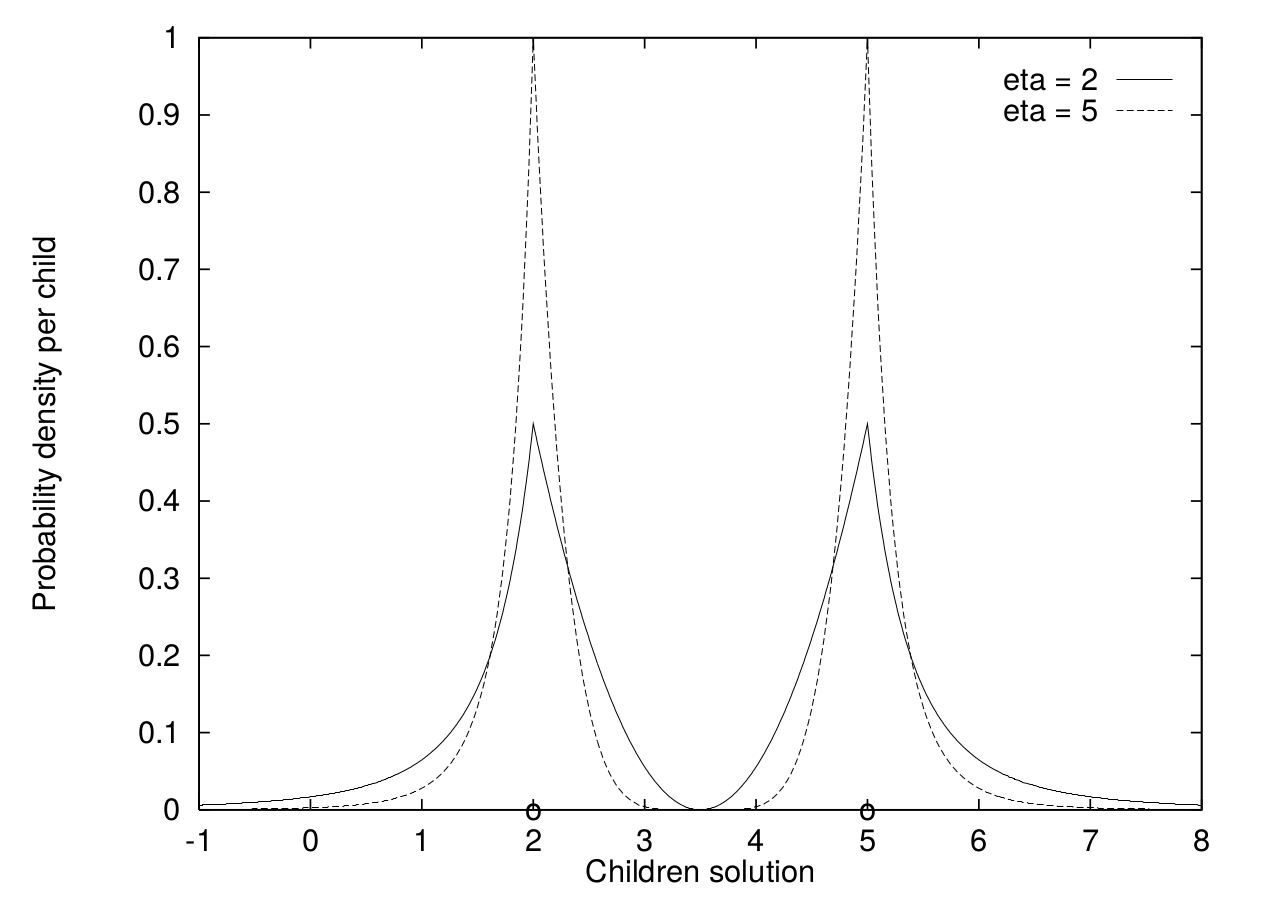
\includegraphics[width=2.5in]{img/Operadores/DensitySBX_English.png}
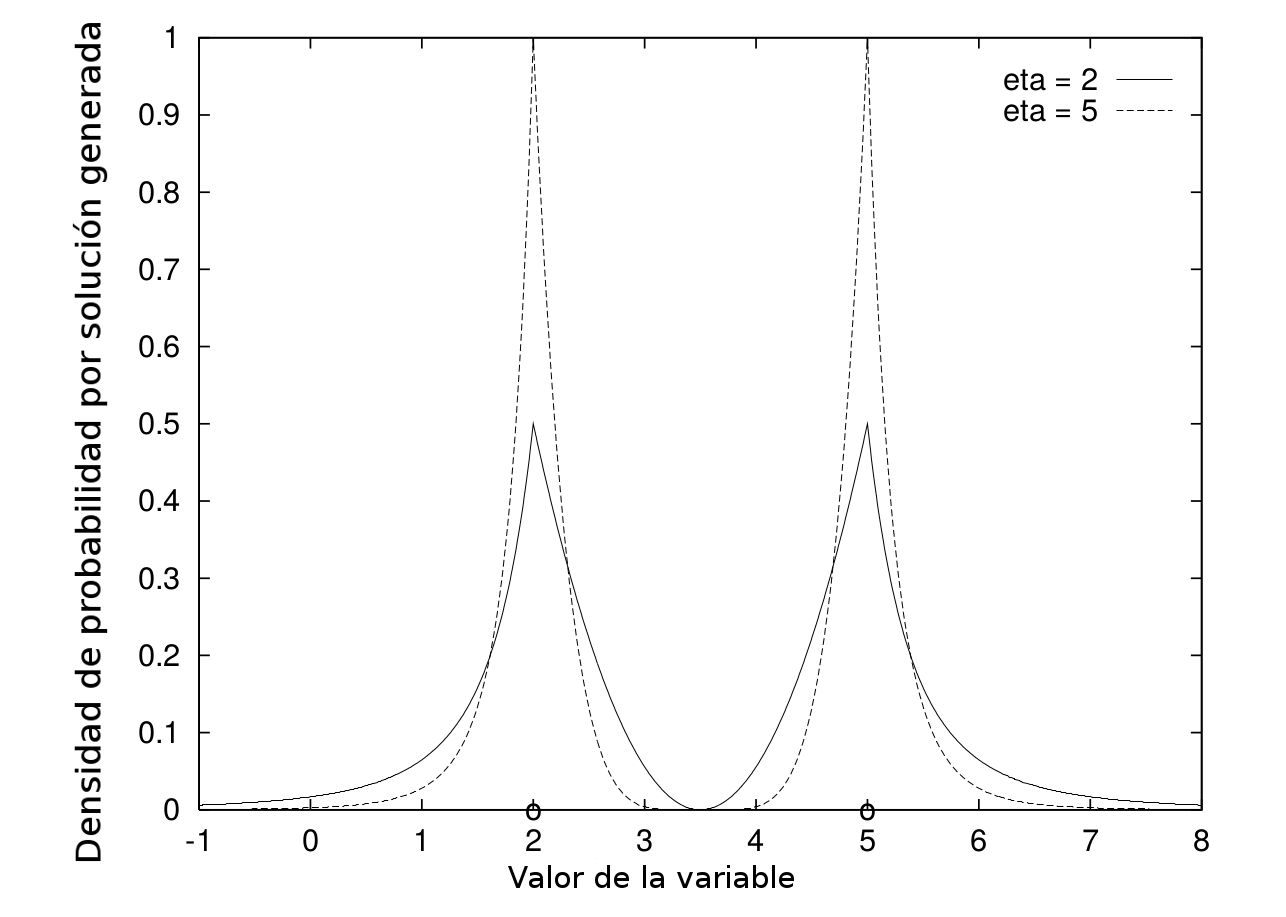
\includegraphics[width=0.5\textwidth]{img/Operadores/DensitySBX.png} 
\caption{Función de densidad del operador de cruce \SBX{} con índices de distribución $2$ y $5$. Las soluciones padre estan ubicadas en $2$ y $5$ respectivamente.}
\label{fig:fig_sim}
\end{figure}

\begin{figure}[!t]
\centering
\begin{tabular}{cc}
   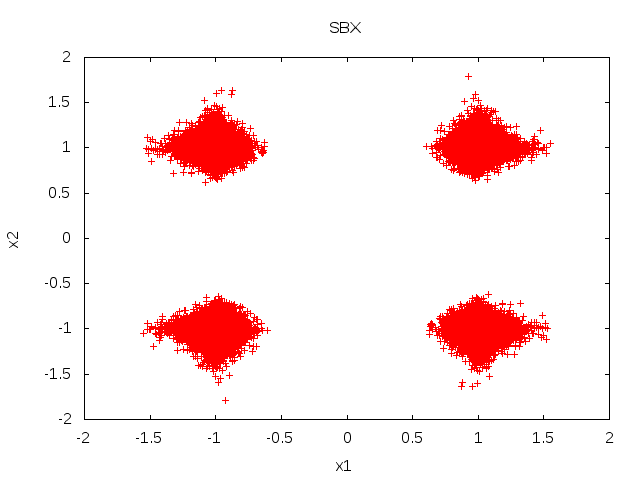
\includegraphics[width=0.35\textwidth]{img/Operadores/SBX_eta_20_2D_pv_1.png} 
   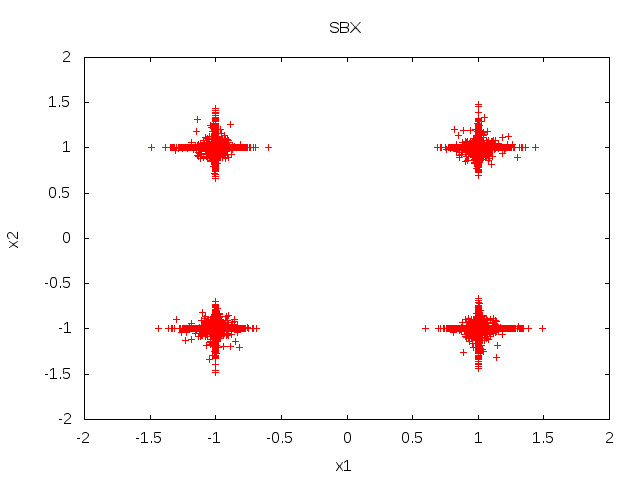
\includegraphics[width=0.35\textwidth]{img/Operadores/SBX_eta_20_2D_pv_01.png} 
\end{tabular}
\caption{Simulaciones de operador \SBX{} con un índice de distribución de $20$. Las soluciones padre están ubicadas en $P_1=(-1.0, -1.0)$ y $P_2=(1.0, 1.0)$. En la parte izquierda la simulación consiste en alterar una variable con probabilidad de $1.0$ y en la pare derecha con probabilidad de $0.1$ (parámetro $\delta_1$ en el Algoritmo \ref{alg:SBX_Operator}).}
\label{fig:Simulation_pv}
\end{figure}



%
\begin{figure}[!t]
\centering
\begin{tabular}{cc}
   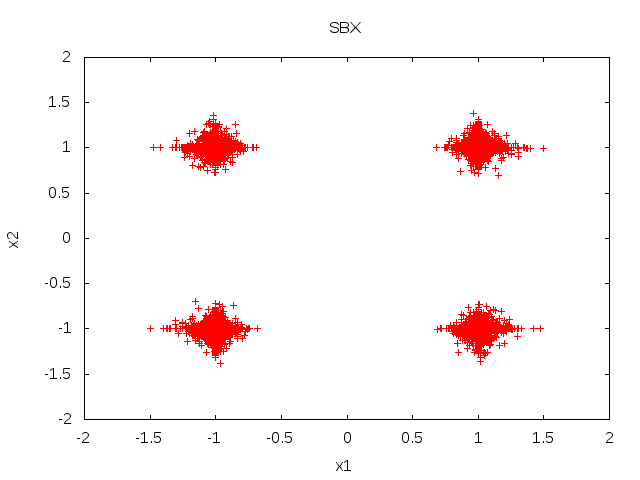
\includegraphics[width=0.35\textwidth]{img/Operadores/SBX_eta_20_2D.png} 
   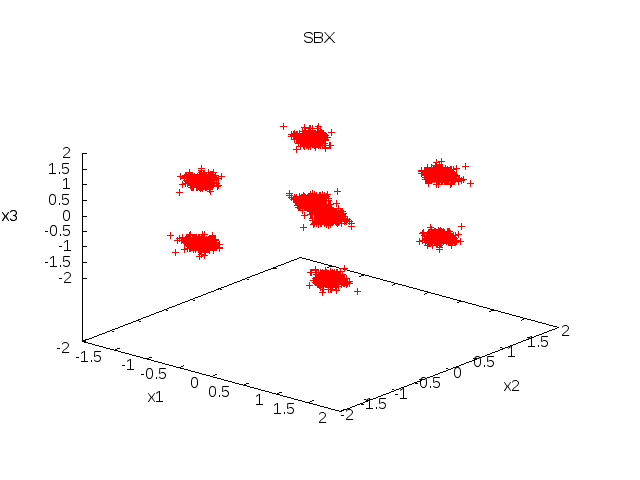
\includegraphics[width=0.35\textwidth]{img/Operadores/SBX_eta_20_3D.png} 
\end{tabular}
\caption{Simulaciones del operador \SBX{} con un índice de distribución de $20$. Las soluciones padre están ubicadas en $P_1=(-1.0, -1.0)$, $P_2=(1.0, 1.0)$ (parte izquierda) y $P_1=(-1.0, -1.0, -1.0)$, $P_2=(1.0, 1.0, 1.0)$ (parte derecha).}
\label{fig:Simulations_Index_20}
\end{figure}


\subsection{Operadores de cruce}
%\subsection{Crossover operators}

Los operadores de cruce son diseñados para generar soluciones hijo utilizando la información de las soluciones padre.
%The crossover operators are designed to generate offspring solutions using information of the parent solutions.
%
Estos combinan las características de dos o más soluciones padre con el propósito de generar nuevas soluciones candidatas.
%They combine features of two or more parent solutions to generate new candidate solutions.
%
En base a que en la literatura existen varios operadores de cruce, se han propuesto varias taxonomías para clasificarlos.
%Since several crossover operators have been proposed, some taxonomies have also been provided.
%
Particularmente, las taxonomías se basan en varias características tales como la ubicación de las nuevas soluciones generadas o por el tipo de relaciones que existen en las variables.
%The taxonomies are based on features such as the location of new generated solutions or the kinds of relations among the variables.

Una taxonomía popular clasifica a los operadores de cruce en \textit{basados en variables} y \textit{basados en vectores}.
%A popular taxonomy classifies crossover operators into variable-wise operators and vector-wise operators.
%
En los \textit{basados en las variables}, cada variable de las soluciones padre son combinadas para crear nuevos valores, esto se realiza de forma independiente y en base a una probabilidad especificada con anterioridad 
%In the variable wise category, each variable from parent solutions is recombined independently with a certain pre-specified probability to create new values.
%
Este tipo de operadores son ideales para lidiar con problemas separables.
%These operators are specially suitable to deal with separable problems.
%
Algunos operadores que pertenecen a esta categoría son el \textit{Operador de Cruce Ciego} (the Blend Crossover - \BLX{})~\cite{eshelman1993real} y el \SBX~\cite{Joel:SBX1994}.
%Some operators belonging to this category are the Blend Crossover (\BLX{})~\cite{eshelman1993real}, and the \SBX{}~\cite{Joel:SBX1994}.
%
De otra forma, los operadores de recombinación \textit{basados en vectores} son diseñados para considerar la dependencia que existe entre las variables.
%Alternatively, the vector-wise recombination operators are designed to take into account the linkage among variables.
%
Este tipo de operadores regularmente realizan una combinación lineal de las soluciones involucradas.
%They usually perform a linear combination of the variable vectors.
%
Algunos operadores que pertenecen a esta categoría son \textit{El Operador de Cruce Unimodal Normalmente Distribuído} (The Unimodal Normally Distributed Crossover - \UNDX{})~\cite{Joel:UNDX}, y \textit{El Operador de Cruce basado en el Simplex} (The simplex crossover - \SPX{})~\cite{Joel:DE_Storn_SPX}.
%Some operators belonging to this category are the Unimodal Normally Distributed Crossover (\UNDX{})~\cite{Joel:UNDX}, and the simplex crossover (\SPX{}) \cite{Joel:DE_Storn_SPX}.
%
Adicionalmente, los operadores de cruce pueden ser clasificados como \textit{basados en los padres} y \textit{basados en la media} \cite{jain2011parent}.
%Additionally, crossover operators can be classified as Parent-Centric and Mean-Centric \cite{jain2011parent}.
%
En los operadores basados en los padres, las soluciones hijo son creadas alrededor de cada solución padre, mientras que en los operadore basados en la media existen una tendencia de crear a las soluciones hijo alrededor de la media generada por las soluciones padres.
%In Parent-Centric operators, children solutions are created around one of the parent solutions, whereas in Mean-Centric operators, children solutions tend to be created mostly 
%around the mean of the participating parent solutions.
%
Entre los operadores de cruce el \SBX{} es probablemente uno de los más utilizados, por lo tanto esta sección se centra en este operador de cruce.
%Among the crossover operators, \SBX{} is probably the most frequently used operator, so this research focuses on this crossover.

\subsubsection{El Operador de Cruce Basado en Simulación Binaria - SBX}
%\subsubsection{Simulated Binary Crossover - SBX}

Los operadores de reproducción son uno de los componentes mas relevantes para influenciar el proceso de búsqueda en los \EAS{}.
%The reproduction operators are one of the most relevant components that influence the search process of \EAS{}.
%
Específicamente, los operadores de cruce y mutación están altamente relacionados con la diversidad de las soluciones.
%Specifically, the crossover and mutation operators are highly related with the diversity of solutions.
%
Por lo tanto, los operadores afectan significativamente la calidad de las soluciones.
%Hence, the quality of solutions are highly affected by the applied operators.
%

Probablemente \textit{El Operador de Cruce Basado en Simulación Binaria} (Simulated Binary Crossover - \SBX{})~\cite{deb1994simulated} es uno de los operadores más populares en dominios continuos y por lo tanto ha sido utilizado extensamente en muchos \MOEAS{}~\cite{Joel:NSGAII,Joel:SMSEMOA}.
%Simulated Binary Crossover (\SBX{})~\cite{deb1994simulated} is probably the most popular operator for continuous domains and most \MOEAS{} have been extensively
%tested with such an operator\cite{Joel:NSGAII,Joel:SMSEMOA}.
%
El operador \SBX{} es clasificado con un operador basado en los padres, lo cual significa que las soluciones las cuales corresponden a los hijos ($c_1$ y $c_2$) serán creadas alrededor de los valores de las soluciones padre ($p_1$ y $p_2$).
%\SBX{} is classified as Parent-Centric, meaning that two children values ($c_1$ and $c_2$) are created around the parent values ($p_1$ and $p_2$).
%
Específicamente, el proceso para generar los valores de las soluciones hijo se basa en una distribución de probabilidad.
%The process of generating the children values is based on a probability distribution.
%
Esta distribución controla el factor de dispersión $\beta = |c_1 - c_2 | / |p_1 - p_2|$ el cual es definido como la razón entre la dispersión de los valores de las soluciones hijo y los valores de las soluciones padre.
%This distribution controls the spread factor $\beta = |c_1 - c_2 | / |p_1 - p_2|$ defined as the ratio between the spread of the children values and parent values.
%
Además, esta función de densidad se define en base a un índice de distribución $\eta_c$ (es un parámetro de control especificado por el usuario) el cual altera la capacidad de exploración.
%In order to define this density function a distribution index $\eta_c$ (a user-defined control parameter) alters the exploration capability of the operator.
%
Especificamente, un índice pequeño induce una probabilidad elevada de crear valores de las soluciones hijo distantes de los valores de las soluciones padre.
%Specifically, a small index induces a larger probability of building children values distant to the parent values, 
Mientras que índices elevados tienden a crear soluciones muy similares a las soluciones padre, esto se demuestra en la Figura~\ref{fig:fig_sim}.
%whereas high indexes tend to create solutions very similar to the parents as is shown in Figure~\ref{fig:fig_sim}.
%

%
Particularmente, para crear una solución hijo se utiliza una distribución de probabilidad la cual está en función de $\beta \in [0, \infty]$ de la siguiente forma:
%The probability distribution to create an offspring value is defined as a function of $\beta \in [0, \infty]$ as follows:
%
\begin{equation}
    P(\beta)= 
\begin{cases}
     0.5(\eta_c + 1)\beta^{\eta_c},& \text{si} \quad \beta \leq 1\\
     0.5(\eta_c + 1) \frac{1}{\beta^{\eta_c + 2}} ,& \text{de otra forma}
\end{cases}
\end{equation}
%
Basado en la propiedad de preservar la media en los valores que corresponden a las soluciones hijo y padre, el \SBX{} tiene las siguientes características:
%Based in the mean-preserving property of children values and parent values, \SBX{} has the following properties:
\begin{itemize}
\item Los valores de las soluciones hijo son equidistantes de los valores de las soluciones padre.
%\item Both offspring values are equi-distant from parent values.
\item Existe una probabilidad no nula de crear soluciones hijo en el espacio factible entero por cualquier par de soluciones padre.
%\item There exist a non-zero probability to create offspring solutions in the entire feasible space from any two parent values.
\item La probabilidad general de crear un par de soluciones hijo dentro del rango de las soluciones padre es idéntico a la probabilidad general de crear un par de soluciones hijo fuera del rango de las soluciones padre.
%\item The overall probability of creating a pair of offspring values within the range of parent values is identical to the overall probability of creating two offspring values outside  
%the range of parent values.
\end{itemize}

Por lo tanto, considerando dos valores de las soluciones padre ($p_1$ y $p_2$) se pueden crear dos valores de las soluciones hijo ($c_1$ y $c_2$) en base a una combinación lineal de los valores de las soluciones padre y con un número aleatorio uniforme $u \in [0, 1]$, especificado a continuación:
%Therefore, considering two participating parent values ($p_1$ and $p_2$), two offspring values ($c_1$ and $c_2$) can be created as linear combination of parent values with a uniform random number $u \in [0, 1]$, as follows:
\begin{equation} 
\begin{split}
c_1 &= 0.5(1 + \beta(u))p_1 + 0.5(1 - \beta(u)) p_2 \\
c_2 &= 0.5(1 - \beta(u))p_1 + 0.5(1 + \beta(u)) p_2
\end{split}
\end{equation}

El parámetro $\beta(u)$ depende en el número aleatorio $u$ de la siguiente forma:
%The parameter $\beta(u)$ depends on the random number $u$, as follows:
\begin{equation}
    \beta(u)= 
\begin{cases}
     (2u)^{\frac{1}{\eta_c+1}},& \text{si} \quad u \leq 0.5,\\
     	(\frac{1}{2(1-u)})^{\frac{1}{\eta_c +1}} ,& \text{de otra forma}
\end{cases}
\end{equation}

La ecuación anterior es formulada en base a un problema de optimización sin límites en las variables.
%The above equation considers an optimization problem with no variable bounds.
%
Sin embargo, en problemas prácticos cada variable es limitada dentro de un límite inferior y superior.
%In most practical problems, each variable is bounded within a lower and upper bound.
%
Por lo tanto, para considerar los límites del espacio de decisión ~\cite{deb1999self} propusieron una modificación de la distribución de probabilidad en la ecuación (\ref{eq:sbx_spread}).
%Thus, the modification of the probability distribution shown in Equation~(\ref{eq:sbx_spread}) 
%was proposed~\cite{deb1999self} with the aim of taking into account such bounds.
%
Es importante resaltar que esta última variante es una de las más utilizadas.
%This last variant is extensively used nowadays.

%
\begin{equation} \label{eq:sbx_spread}
    \beta(u)= 
\begin{cases}
     (2u(1-\gamma))^{\frac{1}{\eta_c+1}},& \text{si} \quad u \leq 0.5/(1-\gamma),\\
     	(\frac{1}{2(1-u(1-\gamma))})^{\frac{1}{\eta_c +1}} ,& \text{de otra forma}
\end{cases}
\end{equation}
\begin{equation} \label{eq:child_1}
c_1 = 0.5(1 + \beta(u))p_1 + 0.5(1-\beta(u))p_2
\end{equation}
\begin{equation} \label{eq:child_2}
c_2 = 0.5(1 + \beta(u))p_1 + 0.5(1-\beta(u))p_2
\end{equation}

En este caso, mediante la Ecuación (\ref{eq:child_1}) se calcula el valor de la solución hijo $c_1$ la cual está más cercana a $p_1$.
%In this case, the child $c_1$ which is nearest to $p_1$ is calculated according to the Equation (\ref{eq:child_1}).
%
Considerando que $p_1 < p_2$ y además con un límite inferior igual a $a$, se tiene que $\gamma = 1/(\alpha^{\eta_c + 1})$, donde $\alpha = 1 + (p_1 - a) / (p_2 - p_1)$.
%Considering that $p_1 < p_2$ and with a lower bound equal to $a$, $\gamma = 1/(\alpha^{\eta_c + 1})$, where $\alpha = 1 + (p_1 - a) / (p_2 - p_1)$.
%
Similarmente, el segundo valor de la solución hijo $c_2$ se calcula con $\alpha = 1 + (b-p_2)/(p_2 - p_1)$, donde $b$ corresponde al límite superior.
%Similarly, the second child $c_2$ is computed with $\alpha = 1 + (b-p_2)/(p_2 - p_1)$, where $b$ correspond to the upper bound.
%
Entonces, el segundo valor de la solución hijo se calcula como se indica en la Ecuación (\ref{eq:child_2}).
%Then, the second child is computed as is indicated in Equation (\ref{eq:child_2}).

\begin{algorithm}[t]
\algsetup{linenosize=\tiny}
\scriptsize
\caption{Operador de Cruce basado en Simulación Binaria (\SBX{})}
%\caption{Simulated Binary Crossover (\SBX{})}
\label{alg:SBX_Operator}
\begin{algorithmic}[1]
    \STATE Entrada: Soluciones padre ($P_{1}, P_{2}$), Indice de distribución ($\eta_c$), Probabilidad de cruce ($P_c$).
    %\STATE Input: Parents ($P_{1}, P_{2}$), Distribution index ($\eta_c$), Crossover probability ($P_c$).
    \STATE Salida: Soluciones hijo ($C_{1}, C_{2}$).
    %\STATE Output: Children ($C_{1}, C_{2}$).
    \IF{ $U[0, 1] \leq P_c$}
       \FOR{para cada variable $d$}
       %\FOR{ each variable d}
	\IF{ $U[0, 1] \leq  \delta_1$} \label{alg:inherit_variable}
		\STATE Generar $C_{1,d}$ utilizando las ecuaciones (\ref{eq:sbx_spread}) y (\ref{eq:child_1}).
		%\STATE Generate $C_{1,d}$ with Equations (\ref{eq:sbx_spread}) and (\ref{eq:child_1}).
		\STATE Generar $C_{2,d}$ utilizando las ecuaciones (\ref{eq:sbx_spread}) y (\ref{eq:child_2}).
		%\STATE Generate $C_{1,d}$ with Equations (\ref{eq:sbx_spread}) and (\ref{eq:child_1}).
		 \IF{$ U[0, 1]  \leq  (1 - \delta_2) $} 
			\STATE Intercambiar $C_{1,d}$ con $C_{2,d}$.
		 \ENDIF
        \ELSE
	   \STATE $C_{1,d} = P_{1, d}$.
	   \STATE $C_{2,d} = P_{2, d}$.
        \ENDIF
       \ENDFOR
    \ELSE
	\STATE $C_{1} = P_{1}$.
	\STATE $C_{2} = P_{2}$.
    \ENDIF
\end{algorithmic}
\end{algorithm}

Es importante aclarar que la primer versión del \SBX{} fue diseñada en base a una sola variable, posteriormente los autores consideraron aplicarlo a problemas con múltiples variables~\cite{Joel:SBX1994}.
%Note that as reported in~\cite{Joel:SBX1994} several extensions of the \SBX{} to problems with multiple
%variables might be provided.
%
Para esto los autores consideraron una estrategia simple para escoger las variables que se van a cruzar~\cite{Joel:UNDX}.
%Authors considered a simple strategy for choosing the variables to cross~\cite{Joel:UNDX}.
%
Específicamente, en base a los principios del operador de cruce unifome cada variable es cruzada con una probabilidad de $0.5$.
%Specifically, each variable is crossed with probability 0.5, following the principles of uniform crossover.
%
Sin embargo, los autores reconocieron las implicaciones que existen con los problemas con dependencia entre las variables.
%Authors recognized the important implications on the linkage among variables of such decisions.
%
En cualquier caso, actualmente ésta es la forma mas común de aplicar el \SBX{} en problemas con múltiple varibles.
%In any case, this is the most typical way of applying \SBX{} in problems with multiple variables nowadays.
%

\subsubsection{Implementación y análisis del operador \SBX{}}
%\subsubsection{Implementation and analyses of SBX operator}

En este apartado se discuten algunas de las principales características de la implementación más utilizada del operador \SBX{}.
%This section discusses some of the main characteristics of the most currently used implementation of the \SBX{} operator for problems with multiple variables.
%
Escencialmente, se consideran tres componentes clave los cuales podrían afectar el rendimiento de los \MOEAS{}.
%Essentially, three key components that might affect its performance are discussed.
%
Primeramente, cada variable es alterada dada una probabilidad de $0.5$.
%Firstly, as already mentioned it alters each variable with a fixed probability equal to $0.5$.
%
Si este valor de probabilidad se incrementa entonces existe una tendencia de generar valores de la solución hijo mas distantes de los padres debido a que mas variables son modificadas por cada operación.
%If this probability value is increased, the children tend to be more distant to the parents, since in average 
%more variables are modified simultaneously.
%
De acuerdo a esto, sería adecuado modificar una variable en los problemas separables.
%In separable problems, altering only one variable might be adequate.
%
Por otra parte, parece ser mas conveniente modificar un conjunto de variables de forma simulánea en problemas no-separables.
%However, for non-separable problems altering several variables simultaneously seems more promising.
%
En la figura~\ref{fig:Simulation_pv} se pueden observar las implicaciones al variar esta probabilidad considerando un problema con dos variables.
%The implications of varying this probability is illustrated in Figure~\ref{fig:Simulation_pv}, where a problem
%with two variables is taken into account.
%
Particularmente, en la parte derecha se muestra que una probabilidad pequeña provoca una tendencia de exploración ya algunas variables no son modificadas, es decir hay una tendencia de generar desplazamientos paralelos a los ejes.
%In the right side a low probability is used and it provokes a bias to explore by keeping some values intact
%creating a figure similar to a cross in the two-dimensional case.
%
Esta característica es ideal para problemas separables.
%This feature might be suitable for separable problems.
%
Por otra parte, en la parte izquierda se muestra que utilizando una probabilidad elevada existe un comportamiento de búsqueda distinto donde la tendencia anterior desaparece, lo cual podría ser ideal para problemas no separables.
%Alternatively, the left side shows that when using a high probability this bias disappears, which could be 
%more suitable for non-separable problems.
%
Es importante destacar que existe una relación entre esta probabilidad y con el índice de distribución, de hecho estos dos factores tienen un efecto directo en la similitud que existe entre las soluciones padre e hijo.
%Note that this probability is somewhat related with the distribution index in the sense that both have a
%direct effect on the similarity between parents and children.
%
%Otherwise, a low probability value is suitable for objective functions that are separable \cite{ma2016multiobjective}, due that few decision variables are modified by the crossover operation.
%
\begin{figure}[t]
\centering
\begin{tabular}{c}
   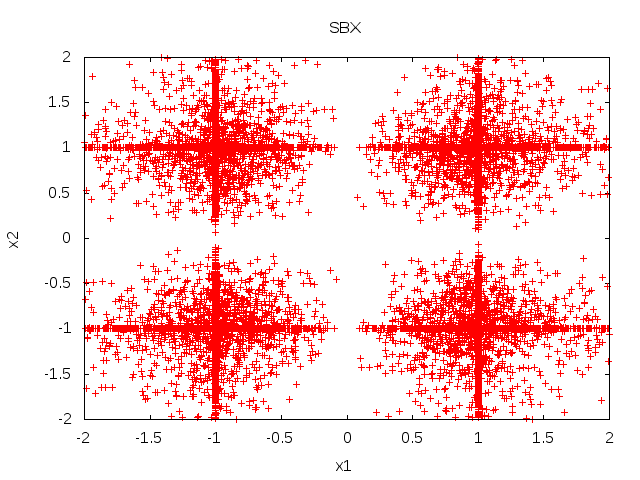
\includegraphics[width=0.35\textwidth]{img/Operadores/SBX_eta_2.png}  %&
   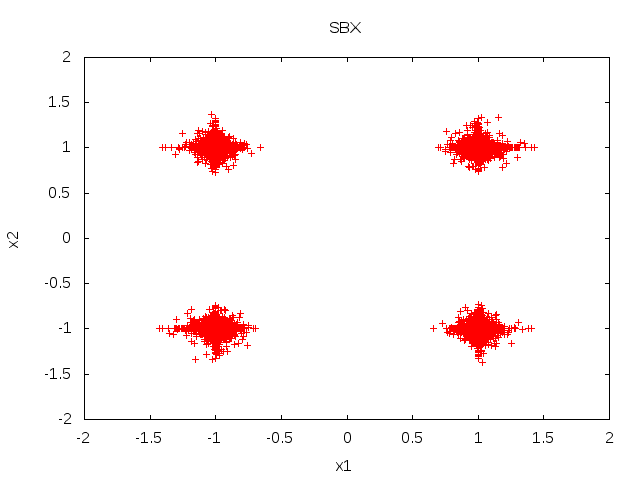
\includegraphics[width=0.35\textwidth]{img/Operadores/SBX_eta_20.png} 
\end{tabular}
\caption{Simulación del operador \SBX{} donde las soluciones padre están ubicadas en $P_1=(-1.0, -1.0)$ y $P_2=(1.0, 1.0)$. En la parte izquierda se consideró un índice de distribución de $2$ y en la derecha de $20$.}
\label{fig:Simulation_Case_3}
\end{figure}

El segundo aspecto importante es al final de aplicar el operador \SBX{} (después de generar dos valores de las soluciones hijo con la distribución), en esta parte los valores son intercambiados con una probabilidad fija (usualmente es $0.5$), es decir el valor de la solución hijo $c_1$ no siempre es heradado por la solución padre más cercana $p_1$.
%The second key issue is that after generating the two child values with the \SBX{} distribution, such values
%are interchanged with a fixed probability that is usually set to $0.5$, i.e. the value closer to parent $p_1$ is
%not always inherited by $c_1$.
%
Esta es una característica no muy discutida, sin embargo es un aspecto muy relevante y afecta al rendimiento del algoritmo.
%This is a feature that is not usually discussed but it is important for the obtained performance.
%
En algunos contextos esta probabilidad se identifica como ``Probabilidad de cruce uniforme por variable'' (Variable uniform crossover probability) \cite{tuvsar2007differential} o ``Recombinación Discreta'' (Discrete Recombination) \cite{muhlenbein1993predictive}.

%In some contexts this probability is known as ``Variable uniform crossover probability'' 
%\cite{tuvsar2007differential} or ``Discrete Recombination'' \cite{muhlenbein1993predictive}.
%
Desde que en el ámbito multi-objetivo se promueve más diversidad en las variables de decision de forma implícita, estos intercambios podrían ser altamente disruptivos.
%Since in multi-objective optimization more diversity is maintained these swaps might produce a high disruptive operator.
%
De hecho, debido a esto, no es totalmente claro que el \SBX{} pueda ser categorizado como un operador totalmente basado en los padres.
%In fact, in some sense due to this action it is not so clear that \SBX{} can be categorized as a parent-centric operator.
%
Estos intercambios que existen entre los valores de las soluciones hijo tienen un efecto de realizar múltiples ``reflexiones'' en el espacio de búsqueda.
%These interchanges between the children has the effect of performing multiple ``reflections'' in the search space.
%
De hecho, conforme incrementa la dimensionalidad en el espacio de las variales, el número de regiones cubiertas incrementa de forma exponencial como se puede observar en los casos de dos y tres dimensiones en la figura \ref{fig:Simulations_Index_20}.
%When increasing the dimensions of the decision variables the number of regions covered increases exponentially 
%as is illustrated in Figure \ref{fig:Simulations_Index_20} where cases with two and three decision variables are taken into account.
%
Es importante notar que esta característica tiene un efecto relevante en la distancia entre las soluciones padre y las soluciones hijo.
%Note also that this feature has a considerable effect on the distance between parents and offspring.

Finalmente, se discute el índice de distribución que es quizás la característica mas conocida del operador \SBX{}.
%Finally, the last component is the distribution index, which is probably the most well known feature of the \SBX{}.
%
Un índice de distribución pequeño provoca un grado de exploración elevado.
%A low index results in greater exploration levels.
%
De hecho, un índice de distribución de la unidad tiene un efecto similar al \textit{Operador de Recombinación Difusa} (Fuzzy Recombination Operator) \cite{voigt1995fuzzy}.
%In fact, a distribution index equal to one has a similar effect to the Fuzzy Recombination Operator \cite{voigt1995fuzzy}.
%
En la figura~\ref{fig:Simulation_Case_3} se puede observar el efecto de aplicar distintos índices de distribución.
%
Particularmente, en la parte izquierda se considera un índice de distribución pequeño, mientras en la parte derecha se considera un índice de distribución grande, se observa que este último genera soluciones candidatas similares a las soluciones padre.
%The effect of applying different indexes is illustrated in Figure~\ref{fig:Simulation_Case_3} where the left side
%considers a low index value whereas the right side takes into account a higher index value, which creates 
%new candidate solutions that are more similar to the parents.
%

En el algoritmo \ref{alg:SBX_Operator} se muestra la implementación del operador \SBX{}.
%The \SBX{} implementation is shown in Algorithm \ref{alg:SBX_Operator}.
%
Este pseudocódigo está basado en la implementación que está integrado en el código del \NSGAII{} propuesto por Deb et al.~\cite{Joel:NSGAII}, la cual se considera como la variante más popular.
%This pseudocode is based on the implementation that is integrated in the NSGA-II code published by Deb et al. \cite{Joel:NSGAII} and which
%is the most popular variant nowadays.
%
En los parámetros de entrada se requieren dos soluciones padre ($P_1$, $P_2$), y éste crea dos soluciones hijo ($C_1$, $C_2$).
%As an input it requires two parents ($P_1$ and $P_2$) and it creates two children ($C_1$ and $C_2$).
%
El primero y el segundo componente mencionados previamente corresponden a las líneas 5 y 9 respectivamente.
%The first and second key components commented previously correspond to the lines 5 and 8, respectively. 
%
Como es usual, el caso clásico del operador \SBX{} se configura con los parámetros $\delta_1 = \delta_2 = 0.5$ y $\eta_c = 20$.
%As is usual, for the basic case, \SBX{} is configured with $\delta_1 = \delta_2 = 0.5$ and $\eta_c = 20$.
%
Es importante notar que la implementación clásica no considera la dimensionalidad en las variables o el criterio de paro como parte de sus parámetros internos.
%It is important take into account that this implementation does not consider the dimension of the decision variables 
%or the stopping criteria to set any of its internal parameters.

\subsection{Propuesta - \DSBX{}}

Basado en el análisis anterior y con el propósito de inducir un balance entre exploración e intensificación, se proponen las siguiente modificaciones.
%Based on the previous analyses and with the aim of inducing an appropriate balance between 
%exploration and intensification, the following modifications are proposed.
%
Primeramente, se modifica la probabilidad de alterar una variable ($\delta_1$) durante la ejecución de forma dinámica.
%First, the probability to modify a variable ($\delta_1$) is dynamically
%modified during the execution.
%
La intención de esta modificación es incrementar la capacidad de exploración en las primeras etapas alterando un conjunto de variables de forma simultánea y conforme la execución procede se reduce el número de variables que son modificadas.
%The rationality behind this modification is to increase the exploration capability in the initial stages
%by altering simultaneously several variables and then, as the evolution proceeds reduce the number of variables
%that are modified.
%
El valor de $\delta_1$ se cambia en base a un modelo lineal decreciente, donde inicialmente se fija a $1.0$ y entonces se decrementa hasta la mitad del total de generaciones con un valor de $0.5$.
%The value of $\delta_1$ is changed in base of a linear decreasing model, where initially it is fixed to $1.0$ and 
%then it is decreased so that at the half of total generations is equal to $0.5$.
%
Esta último valor es mantenido hasta el final de la ejecución, es decir desde la mitad de la ejecución este parámetro se comporta similar a la implementación tradicional del \SBX{}.
%This last value is maintained until the end of the execution, i.e. from the half of the execution it behaves as the 
%traditional \SBX{} implementation.
%

Para asignar el valor $\delta_1$ se utiliza la Ecuación (\ref{eqn:linear}), donde $G_{Transcurridas}$ corresponde a la generación actual y $G_{Total}$ corresponde al número total de generaciones.
%Equation (\ref{eqn:linear}) is the one used to set the value of $\delta_1$, where $G_{Elapsed}$ is the current generation 
%and $G_{End}$ is the total number of generations.

Similarmente, el segundo cambio está relacionado con la probabilidad de aplicar reflexiones ($1 - \delta_2$).
%In a similar way, the second change is related to the probability of performing reflections ($1 - \delta_2$).
%
En este caso $\delta_2$ es actualizado de acuerdo a la Ecuación (\ref{eqn:linear}), por lo tanto la probabilidad de aplicar una reflexión incrementa de $0.0$ a $0.5$ durante la ejecución.
%In this case $\delta_2$ is also updated as in Equation (\ref{eqn:linear}), meaning that the probability of performing
%a reflection increases from $0.0$ to $0.5$ during the execution.
%
Esta modificación se realiza con el propósito de evitar el comportamiento disruptivo de intercambiar variables en las primeras generaciones ya que esto provocaría modificaciones muy drásticas.
%This modification is performed with the aim of avoiding the disruptive behavior of interchanging the variables at the
%first generations because this might result in very drastic modifications.
%
De esta forma, sería mas sensato aplicar estas reflexiones una vez que los individuos convergen a cierto grado.
%Once that the individuals converge to certain degree it might make more sense to perform such reflections.
%
Por lo tanto, esta probabilidad es incrementada a $0.5$, siendo el valor utilizando en la implementación del \SBX{} estándar.
%Thus, this probability is increased to $0.5$ which is the value used in the standard implementation of \SBX{}.

\begin{equation}\label{eqn:linear}
	\delta_1 = \delta_2 = max \left (0.5, 1.0 - \frac{G_{Transcurridas}}{G_{Total}} \right )
\end{equation}

Finalmente, el índice de distribución también es modificado durante la ejecución.
%Finally, the distribution index is also changed during the execution. 
%
De esta forma, en la primeras etapas se promueve un índice de distribución pequeño con el propósito de incrementar la capacidad de exploración del \SBX{}.
%At the first stages a low distribution index is induced with the aim of increasing the exploration capabilities 
%of \SBX{}.
%
Posteriormente se decrementa de forma lineal, lo cual tiene el efecto de que la curva de distribución se cierre, por lo tanto se promueve un mayor grado de intensificación en las etapas finales.
%Then, it is linearly incremented which has the effect of closing the distribution curve, meaning that more intensification is
%promoted.
%
El incremento lineal es indicado en la Ecuación (\ref{eqn:index_eta}), por lo tanto el índice de distribución es alterado de $2$ a $22$.
%The linear increment is governed by Equation (\ref{eqn:index_eta}), meaning that the distribution index is altered
%from $2$ to $22$.
%
Es importante aclarar que ya se han considerado modificaciones similares al índice de distribución \cite{zitzler1999multiobjective}, \cite{hamdan2012distribution}.
%Note that modifications similar to this last one have been explored previously 
%\cite{zitzler1999multiobjective}, \cite{hamdan2012distribution}.
%

\begin{equation}\label{eqn:index_eta}
 \eta_c = 2 + 20 \times \left ( \frac{G_{Elapsed}}{G_{End}} \right)
\end{equation}

\subsection{Resultados}

\begin{table}[t]
\centering
\scriptsize
\caption{Puntos de referencias para el indicador HV}
%\caption{References points for the HV indicator}
\label{tab:ReferencePoints}
\begin{tabular}{cc}
\hline
\textbf{Instancias} & \textbf{Punto de referencia} \\ \hline
%\textbf{Instances} & \textbf{Reference Point} \\ \hline
WFG1-WFG9 & $[2.1, ...,2m+0.1]$ \\
DTLZ 1, 2, 4 & $[1.1, ..., 1.1]$ \\
DTLZ 3, 5, 6 & $[3, ..., 3]$ \\
DTLZ7 & $[1.1, ..., 1.1, 2m]$ \\
UF 1-10 & $[2, ..., 2]$ \\ \hline
\end{tabular}
\end{table}


% Please add the following required packages to your document preamble:
% \usepackage{multirow}
% \usepackage{graphicx}
\begin{table*}[t]
\centering

\caption{Información estadística de las métricas considerando dos objetivos}
%\caption{Statistical Information of Metrics with two objectives}
\label{tab:Metrics_2}
\resizebox{\textwidth}{!}{%
\begin{tabular}{|c|c|c|c|c|c|c|c|c|c|c|c|c|c|c|c|c|c|c|}
\hline
\multirow{2}{*}{} & \multicolumn{6}{c|}{NSGA-II} & \multicolumn{6}{c|}{MOEA/D} & \multicolumn{6}{c|}{SMS-EMOA} \\ \cline{2-19} 
 & 1 & 2 & 3 & 4 & 5 & DE & 1 & 2 & 3 & 4 & 5 & DE & 1 & 2 & 3 & 4 & 5 & DE \\ \hline
Average HV & 0.88 & 0.90 & 0.90 & 0.91 & 0.93 & \textbf{0.94} & 0.87 & 0.87 & 0.87 & 0.90 & \textbf{0.91} & \textbf{0.91} & 0.88 & 0.89 & 0.87 & 0.91 & 0.92 & \textbf{0.93} \\ \hline
%Best Counts HV & 2 & 1 & 0 & 1 & 8 & \textbf{11} & 2 & 0 & 2 & 2 & 8 & \textbf{9} & 0 & 1 & 1 & 5 & 6 & \textbf{10} \\ \hline
%\multicolumn{1}{|l|}{Average Best Difference HV} & \multicolumn{1}{l|}{0.068} & \multicolumn{1}{l|}{0.057} & \multicolumn{1}{l|}{0.053} & \multicolumn{1}{l|}{0.039} & \multicolumn{1}{l|}{0.019} & \multicolumn{1}{l|}{\textbf{0.017}} & \multicolumn{1}{l|}{0.053} & \multicolumn{1}{l|}{0.048} & \multicolumn{1}{l|}{0.049} & \multicolumn{1}{l|}{0.024} & \multicolumn{1}{l|}{\textbf{0.013}} & \multicolumn{1}{l|}{0.014} & \multicolumn{1}{l|}{0.074} & \multicolumn{1}{l|}{0.064} & \multicolumn{1}{l|}{0.081} & \multicolumn{1}{l|}{0.045} & \multicolumn{1}{l|}{0.028} & \multicolumn{1}{l|}{\textbf{0.019}} \\ \hline
Average IGD+ & 0.12 & 0.09 & 0.11 & 0.07 & 0.06 & \textbf{0.05} & 0.14 & 0.12 & 0.14 & 0.09 & 0.08 & \textbf{0.07} & 0.13 & 0.11 & 0.14 & 0.08 & 0.07 & \textbf{0.05} \\ \hline
%Best Counts IGD+ & 2 & 1 & 1 & 1 & 8 & \textbf{10} & 3 & 0 & 2 & 3 & 6 & \textbf{9} & 0 & 2 & 0 & 3 & \textbf{9} & \textbf{9} \\ \hline
%\multicolumn{1}{|l|}{Average Best Difference IGD+} & \multicolumn{1}{l|}{0.086} & \multicolumn{1}{l|}{0.052} & \multicolumn{1}{l|}{0.077} & \multicolumn{1}{l|}{0.035} & \multicolumn{1}{l|}{0.021} & \multicolumn{1}{l|}{\textbf{0.016}} & \multicolumn{1}{l|}{0.075} & \multicolumn{1}{l|}{0.059} & \multicolumn{1}{l|}{0.072} & \multicolumn{1}{l|}{0.025} & \multicolumn{1}{l|}{0.019} & \multicolumn{1}{l|}{\textbf{0.008}} & \multicolumn{1}{l|}{0.093} & \multicolumn{1}{l|}{0.071} & \multicolumn{1}{l|}{0.101} & \multicolumn{1}{l|}{0.038} & \multicolumn{1}{l|}{0.030} & \multicolumn{1}{l|}{\textbf{0.017}} \\ \hline
\end{tabular}%
}
\end{table*}

% Please add the following required packages to your document preamble:
% \usepackage{multirow}
% \usepackage{graphicx}
\begin{table*}[t]
\centering
\caption{Información estadística de las métricas considerando tres objetivos}
%\caption{Statistical Information of Metrics with three objectives}
\label{tab:Metrics_3}
\resizebox{\textwidth}{!}{%
\begin{tabular}{|c|c|c|c|c|c|c|c|c|c|c|c|c|c|c|c|c|c|c|}
\hline
\multirow{2}{*}{} & \multicolumn{6}{c|}{NSGA-II} & \multicolumn{6}{c|}{MOEA/D} & \multicolumn{6}{c|}{SMS-EMOA} \\ \cline{2-19} 
 & 1 & 2 & 3 & 4 & 5 & DE & 1 & 2 & 3 & 4 & 5 & DE & 1 & 2 & 3 & 4 & 5 & DE \\ \hline
Average HV & \textbf{0.87} & 0.84 & \textbf{0.87} & \textbf{0.87} & \textbf{0.87} & 0.85 & 0.84 & 0.84 & 0.84 & \textbf{0.86} & \textbf{0.86} & 0.85 & 0.90 & 0.89 & 0.88 & \textbf{0.91} & \textbf{0.91} & \textbf{0.91} \\ \hline
%Best Counts HV & 1 & 2 & 1 & 4 & 4 & \textbf{7} & 1 & 2 & 1 & 2 & 5 & \textbf{8} & 3 & 2 & 0 & 2 & 5 & \textbf{7} \\ \hline
%\multicolumn{1}{|l|}{Average Best Difference HV} & \multicolumn{1}{l|}{0.019} & \multicolumn{1}{l|}{0.047} & \multicolumn{1}{l|}{0.020} & \multicolumn{1}{l|}{\textbf{0.014}} & \multicolumn{1}{l|}{\textbf{0.014}} & \multicolumn{1}{l|}{0.032} & \multicolumn{1}{l|}{0.036} & \multicolumn{1}{l|}{0.041} & \multicolumn{1}{l|}{0.038} & \multicolumn{1}{l|}{0.016} & \multicolumn{1}{l|}{\textbf{0.013}} & \multicolumn{1}{l|}{0.027} & \multicolumn{1}{l|}{0.038} & \multicolumn{1}{l|}{0.038} & \multicolumn{1}{l|}{0.049} & \multicolumn{1}{l|}{\textbf{0.019}} & \multicolumn{1}{l|}{0.027} & \multicolumn{1}{l|}{\textbf{0.019}} \\ \hline
Average IGD+ & 0.13 & 0.16 & 0.13 & \textbf{0.12} & \textbf{0.12} & 0.13 & 0.15 & 0.14 & 0.15 & \textbf{0.11} & \textbf{0.11} & 0.13 & 0.11 & 0.11 & 0.13 & \textbf{0.09} & \textbf{0.09} & 0.13 \\ \hline
%Best Counts IGD+ & 0 & 2 & 2 & 4 & 3 & \textbf{8} & 2 & 2 & 0 & 2 & 4 & \textbf{9} & 1 & 3 & 0 & 3 & 5 & \textbf{7} \\ \hline
%\multicolumn{1}{|l|}{Average Best Difference IGD+} & \multicolumn{1}{l|}{0.029} & \multicolumn{1}{l|}{0.061} & \multicolumn{1}{l|}{0.027} & \multicolumn{1}{l|}{0.023} & \multicolumn{1}{l|}{\textbf{0.020}} & \multicolumn{1}{l|}{0.032} & \multicolumn{1}{l|}{0.053} & \multicolumn{1}{l|}{0.048} & \multicolumn{1}{l|}{0.053} & \multicolumn{1}{l|}{\textbf{0.015}} & \multicolumn{1}{l|}{\textbf{0.015}} & \multicolumn{1}{l|}{0.030} & \multicolumn{1}{l|}{0.047} & \multicolumn{1}{l|}{0.040} & \multicolumn{1}{l|}{0.062} & \multicolumn{1}{l|}{\textbf{0.020}} & \multicolumn{1}{l|}{0.024} & \multicolumn{1}{l|}{0.069} \\ \hline
\end{tabular}%
}
\end{table*}
\begin{table*}[t]
\centering
\caption{Resúmen de las pruebas estadísticas}
%\caption{Summary of Statistical Tests}
\label{tab:statistical_Tests}
\begin{tabular}{|c|c|c|c|c|c|c|c|c|c|c|c|c|c|c|c|}
\hline
\multicolumn{16}{|c|}{NSGA-II} \\ \hline
 & \multicolumn{3}{c|}{1} & \multicolumn{3}{c|}{2} & \multicolumn{3}{c|}{3} & \multicolumn{3}{c|}{4} & \multicolumn{3}{c|}{5} \\ \hline
 & $\uparrow$ & $\downarrow$ & $\longleftrightarrow$ & $\uparrow$ & $\downarrow$ & $\longleftrightarrow$ & $\uparrow$ & $\downarrow$ & $\longleftrightarrow$ & $\uparrow$ & $\downarrow$ & $\longleftrightarrow$ & $\uparrow$ & $\downarrow$ & $\longleftrightarrow$ \\ \hline
\textbf{HV-2obj} & 16 & 29 & 47 & 6 & 61 & 25 & 28 & 19 & 45 & 31 & 23 & 38 & \textbf{54} & 3 & 35 \\ \hline
\textbf{HV-3obj} & 15 & 19 & 42 & 12 & 50 & 14 & 17 & 15 & 44 & \textbf{33} & 10 & 33 & 26 & 9 & 41 \\ \hline
\textbf{IGD-2obj} & 14 & 30 & 48 & 4 & 60 & 28 & 25 & 17 & 50 & 33 & 19 & 40 & \textbf{52} & 2 & 38 \\ \hline
\textbf{IGD-3obj} & 14 & 18 & 44 & 13 & 44 & 19 & 18 & 15 & 43 & \textbf{33} & 15 & 28 & 23 & 9 & 44 \\ \hline
% \end{tabular}
% \end{table*}

% \begin{table*}[]
% \centering
% \caption{My caption}
% \label{my-label}
% \begin{tabular}{|c|c|c|c|c|c|c|c|c|c|c|c|c|c|c|c|}
\hline
\hline
\multicolumn{16}{|c|}{MOEA/D} \\ \hline
 & \multicolumn{3}{c|}{1} & \multicolumn{3}{c|}{2} & \multicolumn{3}{c|}{3} & \multicolumn{3}{c|}{4} & \multicolumn{3}{c|}{5} \\ \hline
 & $\uparrow$ & $\downarrow$ & $\longleftrightarrow$ & $\uparrow$ & $\downarrow$ & $\longleftrightarrow$ & $\uparrow$ & $\downarrow$ & $\longleftrightarrow$ & $\uparrow$ & $\downarrow$ & $\longleftrightarrow$ & $\uparrow$ & $\downarrow$ & $\longleftrightarrow$ \\ \hline
\textbf{HV-2obj} & 15 & 33 & 44 & 10 & 60 & 22 & 25 & 26 & 41 & 39 & 18 & 35 & \textbf{57} & 9 & 26 \\ \hline
\textbf{HV-3obj} & 10 & 22 & 44 & 12 & 39 & 25 & 11 & 19 & 46 & 24 & 10 & 42 & \textbf{38} & 5 & 33 \\ \hline
\textbf{IGD-2obj} & 16 & 31 & 45 & 9 & 60 & 23 & 23 & 27 & 42 & 37 & 17 & 38 & \textbf{57} & 7 & 28 \\ \hline
\textbf{IGD-3obj} & 12 & 22 & 42 & 13 & 43 & 20 & 13 & 24 & 39 & 30 & 9 & 37 & \textbf{40} & 10 & 26 \\ \hline
% \end{tabular}
% \end{table*}

% \begin{table*}[]
% \centering
% \caption{My caption}
% \label{my-label}
% \begin{tabular}{|c|c|c|c|c|c|c|c|c|c|c|c|c|c|c|c|}
\hline
\hline
\multicolumn{16}{|c|}{SMS-EMOA} \\ \hline
 & \multicolumn{3}{c|}{1} & \multicolumn{3}{c|}{2} & \multicolumn{3}{c|}{3} & \multicolumn{3}{c|}{4} & \multicolumn{3}{c|}{5} \\ \hline
 & $\uparrow$ & $\downarrow$ & $\longleftrightarrow$ & $\uparrow$ & $\downarrow$ & $\longleftrightarrow$ & $\uparrow$ & $\downarrow$ & $\longleftrightarrow$ & $\uparrow$ & $\downarrow$ & $\longleftrightarrow$ & $\uparrow$ & $\downarrow$ & $\longleftrightarrow$ \\ \hline
\textbf{HV-2obj} & 9 & 35 & 48 & 7 & 43 & 42 & 16 & 31 & 45 & 41 & 9 & 42 & \textbf{53} & 8 & 31 \\ \hline
\textbf{HV-3obj} & 7 & 21 & 48 & 9 & 35 & 32 & 13 & 21 & 42 & 27 & 6 & 43 & \textbf{31} & 4 & 41 \\ \hline
\textbf{IGD-2obj} & 10 & 34 & 48 & 15 & 48 & 29 & 12 & 33 & 47 & 41 & 12 & 39 & \textbf{55} & 6 & 31 \\ \hline
\textbf{IGD-3obj} & 8 & 20 & 48 & 13 & 30 & 33 & 9 & 19 & 48 & 22 & 5 & 49 & \textbf{27} & 5 & 44 \\ \hline
\end{tabular}
\end{table*}

En este apartado se analizan los resultados obtenidos con las variantes dinámicas del \SBX{} (\DSBX{}).
%This section is devoted to analyze the results obtained with the dynamic variants of \SBX{} (\DSBX{}).
%
Cada uno de los casos préviamente analizados y una propuesta se integraron en los algoritmos \NSGAII{}, \MOEAD{} y \SMSEMOA{}.
%The novel crossover operator was integrated with \NSGAII{}, \MOEAD{} and \SMSEMOA{}.
%
Primeramente, se analiza cada uno de los tres componentes que se analizaron con anterioridad.
%First, three variants that alter only one of each of the components previously discussed are analyzed.
%
Posteriormente se construye un caso donde se consideran dos componentes de forma simultánea.
%Then, a case that alters two of them simultaneously is taken into account.
%
Como parte de la validación experimental se consideran los problemas de prueba WFG \cite{Joel:WFG}, DTLZ \cite{Joel:DTLZ_2} and UF \cite{zhang2009performance}.
%The WFG \cite{Joel:WFG}, DTLZ \cite{Joel:DTLZ_2} and UF \cite{zhang2009performance} test problems have been used for our purpose.
%
Además, con el propósito de comparar nuestra extensión del \SBX{} con otros operadores se incluye evolución diferencial mejor conocidos como \DEMO{}~\cite{tuvsar2007differential}.
%Our experimental validation also includes the variant of Differential Evolution known as DEMO~\cite{tuvsar2007differential}
%with the aim of comparing our extension of \SBX{} with other well-known operators.
Debido a que todos los algoritmos son estocásticos cada ejecución se repitió $35$ veces con distintas semillas.
%Given that all the methods are stochastic algorithms, each execution was repeated $35$ times with different seeds.
%
La configuración global que se aplica a todos los algoritmos se indica a continuación.
%
Se asgina el criterio de paro a $25,000$ generaciones, el tamaño de la población a $100$, se configuraron los problemas de prueba \WFG{} con dos y tres objetivos, además se consideraron 24 variables, donde $20$ variables eran considerados como parámetros de distancia y $4$ se consideraron como parámetros de posición.
%The common configuration in all of them was the following: the stopping criterion was set to $25,000$ generations, 
%the population size was fixed to 100, WFG test problems were configured with two and three objectives, and 24 variables
%were considered, where 20 of them are distance parameters and 4 of them are position parameters.
%
Como es sugerido en \cite{Joel:DTLZ_2} se consideran $n=M+r-1$ variables de decisión en los problemas de prueba \DTLZ{}, donde para los problemas DTLZ1, DTLZ2 - DTLZ6 y DTLZ7 se consideraron $r=\{5, 10, 20\}$  respectivamente.
%In the case of the DTLZ test instances, the number of decision variables were set to $n=M+r-1$, where $r=\{5, 10, 20\}$ 
%for DTLZ1, DTLZ2 to DTLZ6 and DTLZ7 respectively, as is suggested in\cite{Joel:DTLZ_2}.  
% 
Para los problemas de prueba \UF{} se asignaron $10$ variable de decisión.
%In the UF benchmark set the number of decision variables were set to 10.
%
Finalmente, se asignó el operador de mutación polinomial con una probabilidad de cruce de $1/n$ y con un índice de distribución de $50$, mientras que el operador de cruce \SBX{} se asignó con una probabilidad de cruce de $0.9$ y un índice de distribución de $20$.
%Finally, the polynomial mutation was used with a mutation probability equal to $1/n$ and with a distribution index equal to 50, 
%whereas for the cases that used the \SBX{}, the crossover probability was set to $0.9$ and the distribution index
%was set to 20.
%
A continuación se especifica la parametrización adicional de cada algoritmo:
%The additional parameterization of each algorithm was as follows:
\begin{itemize}
\item \textbf{DEMO}: CR = 0.3 and F = 0.5.
\item \textbf{SMS-EMOA}: desplazamiento para calcular el HV = 100.
%\item \textbf{SMS-EMOA}: offset = 100.
\item \textbf{MOEA/D}: tamaño de la vecindad = 10, el número de actualizaciones por subproblema ($nr$) = 2 y $\delta = 0.9$.
i%\item \textbf{MOEA/D}: size of neighborhood = 10, max updates by sub-problem (nr) = 2 and $\delta = 0.9$.
\end{itemize}

Para comparar los frentes obtenidos de cada método se utiliza el hipervolúmen normalizado (HV) y la \textit{Distancia Generacional Invertida Modificada} (Inverted Generational Distance Plus - IGD+).
%In order to compare the fronts obtained by the different methods the 
%normalized hypervolume (HV) and IGD+ was taken into account.
%
En la tabla \ref{tab:ReferencePoints} se presentan los puntos de referencia utilizados para el indicador del hipervolúmen los cuales son similares a los utilizados en \cite{Joel:Kuhn_Munkres, Joel:OperatorAHX}.
%The reference points used for the hypervolume indicator are shown in the Table \ref{tab:ReferencePoints} 
%and are similar to the ones used in \cite{Joel:Kuhn_Munkres, Joel:OperatorAHX}.
%
Por otra parte para comparar los resultados estadísticamente (valores del IGD+ y HV), se siguió un procedimiento similar al que se propuso en~\cite{Joel:StatisticalTest}.
%In order to statistically compare the results (IGD+ and HV values), the following statistical tests were performed. 
%In order to statistically compare the results, a similar guideline than the one proposed in~\cite{Joel:StatisticalTest} was used. 
%
En primer lugar, se utilizó la prueba Shapiro-Wilk para comprobar si los resultados se ajustaban a una distribución Gaussiana. 
%
%First a Shapiro-Wilk test was performed to check whatever or not the values of the results followed a Gaussian distribution. 
%
En los casos en que sí se ajustaban, se utilizó la prueba de Levene para comprobar la homogeneidad de las varianzas, procediendo con la prueba de ANOVA en caso positivo o con el de Welch en caso negativo.
%
%If, so, the Levene test was used to check for the homogeneity of the variances. 
%If samples had equal variance, an ANOVA test was done; if not, a Welch test was performed. 
%
Por otro lado, para los casos que no se ajustaban a distribuciones Guassianas, se utilizó la prueba de Kruskal-Wallis.
%For non-Gaussian distributions, the nonparametric Kruskal-Wallis test was used to test whether samples are drawn 
%from the same distribution. 
%
En todos los casos se fijó el nivel de confianza al 95\%.
%
Se considera que un algoritmo $X$ es superior a un algoritmo $Y$, si el procedimiento anterior reporta diferencias significativas, además si la media y mediana del hipervolumen obtenido por el método $X$ son superiores a las obtenidas por el método $Y$.
%
%An algorithm $X$ is said to win algorithm $Y$ when the differences between them are statistically significant, and
%the mean and median obtained by $X$ are higher (in HV) or lower (in IGD+) than the mean and median achieved by $Y$.


\subsection{Análisis de cada compenente en el operador \SBX{}}
%\subsection{Analysis of isolated components}

En este apartado se analiza el efecto que cada componente tiene de forma independente los cuales son modificador en base a un modelo dinámico.
%In this section we discuss about the independent effect of each component that is dynamically modified.
%
%
Basados en el algoritmo \ref{alg:SBX_Operator} el efecto de cada componente es analizado a través de cuatro casos
%The effect of each component is analyzed through four cases, based in the Algorithm \ref{alg:SBX_Operator}.
%
Cada caso es descrito a continuación.
%Each case is described as follows:

\begin{itemize}
\item \textbf{Caso 1}: Se aplica la versión estańdar del operador \SBX{} donde $\delta_1 = \delta_2 = 0.5$ y $\eta_c = 20$.
%\item \textbf{Case 1}: The standard SBX operator where $\delta_1 = \delta_2 = 0.5$ and $\eta_c = 20$.
\item \textbf{Caso 2}: Se actualiza el valor $\delta_1$ como se indica en la Ecuación~(\ref{eqn:linear}),  $\delta_2=0.5$ y $\eta_c = 20$.
%\item \textbf{Case 2}: The value $\delta_1$ is updated according to Equation~(\ref{eqn:linear}),  $\delta_2=0.5$ and $\eta_c = 20$.
\item \textbf{Caso 3}: Se actualiza el valor $\delta_2$ como se indica en la Ecuación~(\ref{eqn:linear}), $\delta_1=0.5$ y $\eta_c = 20$.
%\item \textbf{Case 3}: The value $\delta_2$ is updated according to Equation~(\ref{eqn:linear}), $\delta_1=0.5$ and $\eta_c = 20$.
\item \textbf{Caso 4}: Se actualiza el índice de distribución de acuerdo a~(\ref{eqn:index_eta}), $\delta_1=\delta_2=0.5$.
%\item \textbf{Case 4}: The distribution index is updated according to Equation~(\ref{eqn:index_eta}), $\delta_1=\delta_2=0.5$.
\end{itemize}

En las tablas \ref{tab:Metrics_2} y \ref{tab:Metrics_3} se muestra información del HV normalizado \cite{zitzler1999multiobjective} y del IGD+ \cite{Joel:IGDPlus_And_GDPlus} para cada caso (Posteriormente se analiza el Caso 5).
%In order to analyze the performance of each Case (Case 5 is discussed later), Tables \ref{tab:Metrics_2} and
%\ref{tab:Metrics_3} shows information about the Normalized Hyper-volume 
%(HV)~\cite{zitzler1999multiobjective} and about the Inverted Generational Distance Plus (IGD+)~\cite{Joel:IGDPlus_And_GDPlus}.
%
Específicamente, se muestra la media del HV e IGD+ para todos los problemas en dos y tres objetivos.
%Specifically, the mean of the HV and IGD+ for all considered problems are shown for two and three objectives.
%
Se observa que considerando dos y tres objetivos el Caso 4 mejora al Caso 1, al Caso 2 y al Caso 3 en todos los algoritmos.
%It is clear that case 4 outperforms case 1, case 2 and case 3 both with two and three objectives in all the tested algorithms.
%
Por lo tanto se aprecian los beneficios de incrementar el índice de distribución durante la ejecución.
%%Therefore, increasing the distribution index during the execution seems to be the most beneficial action.
%
Esto sucede porque inicialmente la curva que corresponde a la distribución de probabilidad conduce a un grado elevado de exploración, mientras que al trancurrir las generaciones se cambia gradualmente a un procedo de intensificación.
%This occurs because the initially open distribution curve leads to a higher degree of exploration, whereas as the evolution
%proceeds more intensification is promoted.
%
Por otra parte, al considerar tres objetivos el Caso 2 presentó un rendimiento menor que al Caso 1.
%On the other hand, case 2 presented a lower performance than case 1 when taking into account three objectives.
%
Por lo tanto, se observa que alterar todas las variables provoca un comportamiento muy disruptivo.
%Thus, it seems that altering almost all the variables convert the new approach into a too disruptive operator.
%
Quizás los resultados podrían mejorar si el parámetro $\delta_1$ es alterado de una forma distinta, sin embargo esto se deja como trabajo futuro.
%Perhaps, altering $\delta_1$ in a different way might provide better results, but this is left as a future work.
Los análisis anteriores únicamente consideran la media obtenida en todos los problemas de prueba.
%Previous analyses are only based on the mean obtained for all the problems.
%
Sin embargo, dependiendo en el tipo de problema el rendimiento del algoritmo podría cambiar.
%However, depending on the problem the performance might vary.
%
Esto se analiza en la siguiente sección.
%This is analyzed in the following section.
%
Adicionalmente, se anexan resultados detallados\footnote{https:\//\//github.com\//joelchaconcastillo\//SBX\_CEC2018.}.
%Additionally, more detailed results are available\footnote{https:\//\//github.com\//joelchaconcastillo\//SBX\_CEC2018.}.


\subsection{Modificación simultánea de varios componentes}
%\subsection{Simultaneous modification of several components}

En base a los resultados obtenidos con anterioridad se propone una variante del operador \SBX{}.
%
En esta variante se incorporan los casos Caso 3 y Caso 4 de forma simultánea, es decir existen un cambio dinámico en el parámetro $\delta_2$ y en el índice de distribución.
%Based on the previously discussed results, a variant of the \SBX{} is proposed where the case 3 and case 4 are mixed, 
%i.e. both $\delta_2$ and the distribution index are updated dynamically.
%
Además, no es considerado el Caso 2 el cual aplica un mecanismo para actualizar $\delta_1$, eso ya que los beneficios con esta variante no fueron significativos.
%Since case 2 did not report significant benefits, the updating mechanism for $\delta_1$ was discarded.
%
Particularmente, el Caso 5 se construye en base al Algoritmo \ref{alg:SBX_Operator} y se configure como se indica a continuación.
%Specifically in our case 5, Algorithm \ref{alg:SBX_Operator} is configured as follows.
%
El parámetro $\delta_1$ es asignado con $0.5$ debido a que es la forma de la versión estándar del \SBX{}.
%The parameter $\delta_1$ is fixed to $0.5$, i.e. in a similar way than the standard \SBX{}.
%
En base al Caso 3, el parámetro $\delta_2$ es actualizado de acuerdo a la Ecuación~(\ref{eqn:linear}).
%Following the case 3, $\delta_2$ is updated according to Equation~(\ref{eqn:linear}).
%
Finalmente, en base al Caso 4, el parámetro $\delta_2$ es actualizado como se indica en la Ecuación (\ref{eqn:index_eta}).
%Finally, according to case 4 $\eta_c$ is updated in base of Equation~(\ref{eqn:index_eta}).

De acuerdo a la media del HV y del IGD+ que se obtuvieron en el Caso 5 (revisar tablas~\ref{tab:Metrics_2} y \ref{tab:Metrics_3}), se pueden observar los beneficios de integrando los Casos 3 y 4.
%Attending to the mean HV and IGD+ obtained by the case 5 (see Tables~\ref{tab:Metrics_2} and \ref{tab:Metrics_3})
%it is clear that integrating case 3 and case 4 is beneficial.
%
En el caso de dos objetivos se observa una ventaja significativa, sin embargo en el caso de tres objetivo los Casos 4 y 5 son muy similares en base a la media.
%The advantages are clearer in the case of two objectives, whereas in the case of three objectives, case 4
%and case 5 are similar in terms of mean performance.
%
Además, al considerar tres objetivos los resultados que se obtuvieron en el Caso 5 son superiores a los obtenidos con \DE{}, mientras que al considerar la versión estándar de \SBX{} se observa un deterioro.
%Moreover, results attained with case 5 are superior to the ones obtained with \DE{} in three objectives, whereas
%when using the traditional \SBX{} results deteriorate.
%
Por lo tanto, si el operador \SBX{} es configurado adecuadamente puede generar resultados similares o superiores que los algoritmos \DEMO{}. 
%Thus, when properly configuring a \DSBX{} results similar or superior to DEMO could be obtained.

Finalmente, debido a que los análisis previos únicamente consideran la media entre la problemas de prueba, a continuación se presenta un análisis adicional para comprender mejor las contribuciones de los distintos casos.
%Finally, since previous analyses only consider the mean among all the benchmark problems, an additional analyses
%was developed to better understand the contributions of the different cases.
%
Particularmente, se realizan comparaciones en pares en base a pruebas estadísticas entre los cinco casos donde es considerado el \SBX{} y \DSBX{}.
%Particularly, pair-wise statistical tests among all the five cases that consider \SBX{} and \DSBX{} were carried out.
%
Este procedimiento se realizó de forma independiente para cada el \NSGAII{}, \MOEAD{} y el \SMSEMOA{}.
%This was performed independently for \NSGAII{}, \MOEAD{} and \SMSEMOA{}.
%
En la tabla ~\ref{tab:statistical_Tests}, se muestra los resultados de las pruebas estadísticas.
%Results of these statistical tests are shown in Table~\ref{tab:statistical_Tests}.
%
Para cada algoritmo y para cada caso, la columna ``$\uparrow$'' reporta el número de comparaciones donde las pruebas estadísticas confirmaron la superioridad del caso correspondiente, mientras que en la columna ``$\downarrow$'' se reporta el número de veces donde este caso fue inferior y la columna ``$\longleftrightarrow$'' indica el número de comparaciones donde la diferencia estadística no fue significativamente distinto.
%For each algorithm and case, the column ``$\uparrow$'' reports the number of comparisons where the statistical tests 
%confirmed the superiority of the corresponding case, whereas the column ``$\downarrow$'' reports the number of cases 
%where it was inferior and ``$\longleftrightarrow$'' indicates the number of comparisons where 
%differences were not statistically significant.
%%
Los beneficios obtenidos por el caso 5 son suficientemente claros.
%The advantages of case 5 are quite clear.
%
Únicamente el Caso 4 obtuvo mejores resultados que el Caso 5 al considerar tres objetivos y al algoritmo \NSGAII{}.
%Only in the case of \NSGAII{} with three objectives, case 4 could outperform the results obtained by case 5.
%
Esto demuestra que se pueden obtener mejores resultados si se integran varias modificaciones dinámicas.
%Thus, by properly combining several dynamic modification, results can be improved further.
%
Principalmente, los resultados confirman varias ventajas al comparar nuestras variantes con la versión estándar del operador \SBX{} (Caso 1).
%Moreover, results confirm the advantages of our proposals when compared to the standard \SBX{} (case 1).
%
El único caso que no es cláramente superior a la versión estándar del \SBX{} es el Caso 2, el cual fue discutido con anterioridad.
%The only case that is not clearly superior to the standard \SBX{} is the case number 2, as it was previously discussed.
%


\section{Conclusiones y trabajo futuro}
\label{sec:Conclusion}
%%%%La convergencia prematura es una de las debilidades más importantes de los \EAS{}.
%
Una de las formas de lidiar con este problema consiste en inducir un balanceo adecuado entre exploración e intensificación.
%
Sin embargo, obtener este balanceo no es una tarea trivial debido a que cada problema de optimización tiene características distintas y por
ello han surgido numerosos esquemas para tratar esta problemática.
%
En base a esto se han desarrollado varias taxonomías con el propósito de clasificar las diferentes formas en que se puede preservar y promover la diversidad.
%
En este trabajo, con el fin de ilustrar como se pueden realizar diseños de \EAS{} que tomen en cuenta el balanceo entre exploración e intensificación
se presentan dos ejemplos.
%
De forma general, las propuestas establecen un comportamiento dinámico de algún componente del \EA{} teniendo en cuenta para ello el criterio de paro 
y el instante en que se encuentra la ejecución.
%
Así se obtuvo un balanceo adecuado en el que en las primeras fases se promueve más exploración y en las últimas más intensificación. 
%
De modo más específico, en la primera propuesta se modifica evolución diferencial por medio de una nueva fase de reemplazo con el propósito de conseguir este balanceo. 
%
Además esta contribución incorpora una población elite con el propósito de proporcionar soluciones de calidad tanto a mediano como a largo plazo.
%
En base a la validación experimental llevada a cabo, se observa que esta propuesta mejora a los mejores algoritmos que se habían propuesto en una competición
que consideró las funciones de prueba usadas en este capítulo.
%
Posteriormente, se presenta un análisis del operador de cruce \SBX{} y se desarrolló una variante que modifica varios componentes de forma dinámica
considerando también el criterio de paro y generaciones transcurridas. 
%
En base a los resultados obtenidos con problemas muy populares del ámbito de optimización multi-objetivo, se muestra que usar el operador \SBX{} modificado ofrece ventajas muy importantes
en varios \MOEAS{} y para diferentes indicadores.
%
De forma general se observa que obtener un balanceo apropiado entre exploración e intensificación es realmente importante, y que
esto se puede conseguir utilizando técnicas radicalmente diferentes aunque siguiendo los mismos principios de diseño.

El campo de diseño de \EAS{} es un campo muy activo y en el que hay muchas ideas aún por explorar.
%
Uno de los aspectos importantes es que este tipo de estrategias ofrecen muchas ventajas a largo plazo, pero se debe hacer el esfuerzo por conseguir
que se pueda reducir lo máximo el número de evaluaciones requeridas para obtener resultados prometedores.
%
Otro aspecto importante es que en general, la mayor parte de estrategias de control de diversidad introduce nuevos parámetros, por lo que es importante
combinar estos mecanismos con estrategias de control de parámetros adaptativas o auto-adaptativas para facilitar su utilización.
%
Finalmente, para el caso específico del \SBX{}, sería interesante integrarlo con técnicas de aprendizaje para lidiar con problemas con dependencias y mejorar
así aún más el rendimiento de la propuesta.


\section*{Agradeciemientos}
Los autores agradecen el apoyo financiero proporcionado por CONACyT a través del proyecto no. 285599.

%\bibliographystyle{spphys}       % APS-like style for physics

\bibliography{InfSci-14-segura}

\end{document}
